\newpage
\section{Результаты и их обсуждение}
\sloppy{
\subsection{Радиолиз бензола}
В ИК-спектрах осаждённых образцов бензола в матрицах аргона, криптона и ксенона присутствуют узкие полосы поглощения,
соответствующие бензолу, их частоты согласуются с литературными данными \cite{Kim1996}. Кроме того, в спектрах осаждённых образцов присутствуют полосы, соответствующие незначительным количествам воды и углекислого газа.
Типичный вид спектра осаждённого образца C$_6$H$_6$/Ng представлен на рисунке~\ref{depAr}.
\begin{figure}[H]
\center{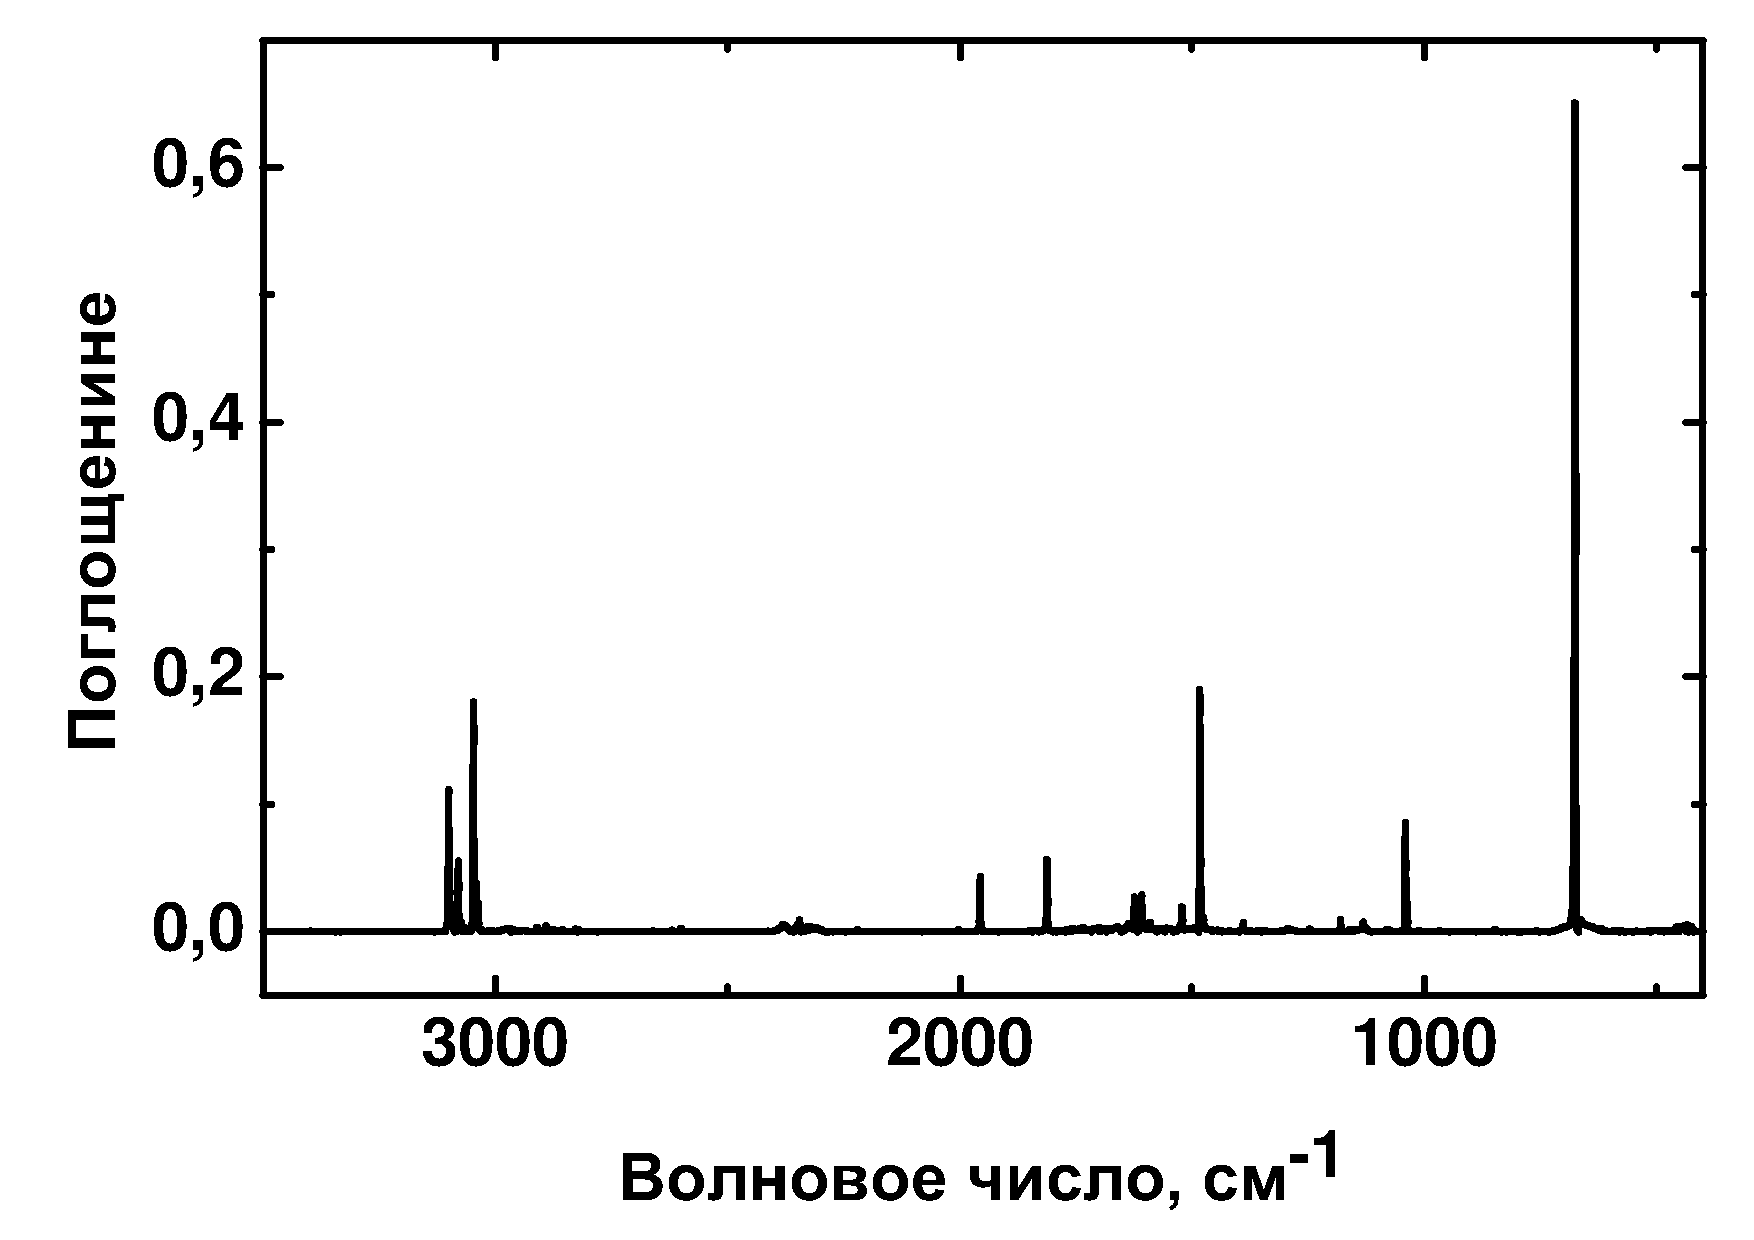
\includegraphics[width=0.9\linewidth]{is.pdf}}
\caption{ИК-спектр осаждённой смеси C$_6$H$_6$/Ar 1:1000}
\label{depAr}
\end{figure}

В результате облучения бензол расходуется во всех матрицах довольно эффективно. Зависимости относительной концентрации бензола (отношение интегральных интенсивностей сигналов
 в облучённом и не облучённом образцах)
  от поглощённой дозы в различных матрицах представлены на рисунке~\ref{conv}.
Использование относительной концентрации бензола в качестве одной из координат позволяет сравнивать результаты, полученные в различных матрицах, без использования коэффициентов 
молярного поглощения, не вносить поправку на различную толщину осаждённого слоя в экспериментах.

\begin{figure}[H]
\center{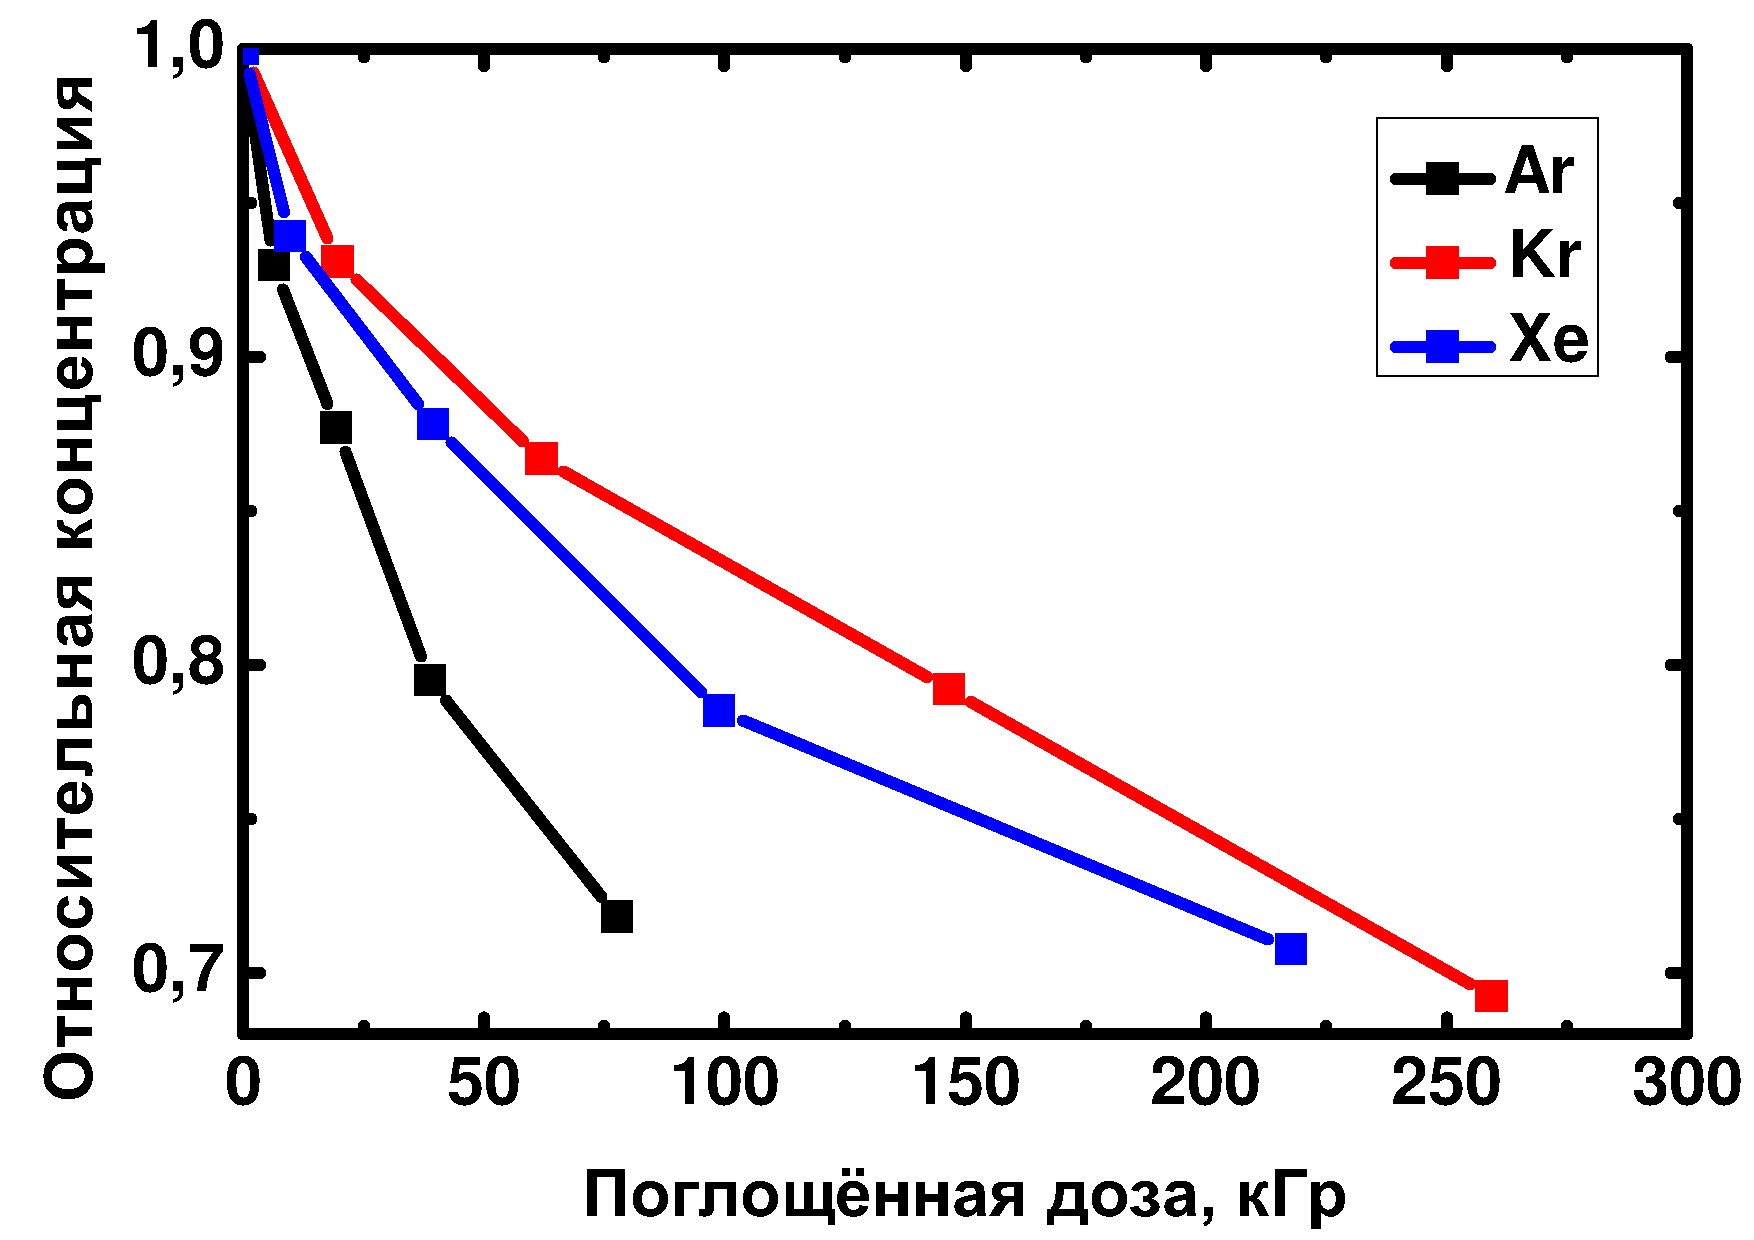
\includegraphics[width=0.8\linewidth]{dose_1.pdf}}
\caption{Кривые расходования бензола в различных матрицах}
\label{conv}
\end{figure}

Разложение бензола в матрице аргона протекает эффективнее, чем в более тяжёлых матрицах (Kr, Xe). Начальные участки всех кривых линейны, при больших дозах (более 100~кГр) в криптоне и ксеноне наблюдается так называемое <<дозовое насыщение>>~---
уменьшение эффективности разложения с увеличением поглощённой дозы. Такой вид зависимости  является типичным для радиолиза большинства веществ, в связи с накоплением продуктов радиолиза и уменьшением концентрации бензола, что снижает эффективность передачи энергии на оставшиеся молекулы бензола. По наклону линейных начальных участков кривых, представленных на рисунке~\ref{conv}, определены радиационно-химические выходы разложения
бензола по формуле:
\begin{equation} \label{yee}
G = \frac{\Delta c}{1000MtI}, 
\end{equation}
где $\Delta c$~--- изменение относительной концентрации бензола, 1000~--- мольное отношение матрицы и бензола, $M$~--- молярная масса матрицы, $t$~--- время облучения, $I$~--- мощность дозы.

Значения выходов составили
2.6~молек./100~эВ в матрице аргона и  0.4~молек./100~эВ в матрицах криптона и ксенона. Радиационно-химический выход разложения бензола сопоставим с 
выходами разложения других молекул в условиях матричной изоляции (см.~раздел~\ref{isolation}), что ставит под вопрос радиационную стойкость бензола, обусловленную его молекулярными свойствами.
 Следует отметить, что радиационно-химический выход разложения бензола в матрицах инертных газов ниже, чем выход разложения бензола при радиолизе в газовой фазе (см.~раздел~\ref{products}), это является типичной ситуацией из-за более лёгкой диссипации энергии в твёрдой фазе по сравнению с газовой.
Понижение выхода разложения бензола при переходе от аргоновой к криптоновой и ксеноновой матрицам, по-видимому, можно объяснить действием двух факторов. 
Во-первых, в тяжёлых матрицах эффективно происходит интеркомбинационная конверсия, из-за чего вклад каналов, 
протекающих через синглетные состояния, значительно уменьшается. Во-вторых, матрицы криптона и ксенона обладают большей поляризуемостью, чем матрица аргона, что приводит
к эффективной релаксации возбуждённых состояний к основному электронному состоянию.


После облучения бензола во всех матрицах в ИК-спектрах появляются новые полосы поглощения (см. рисунок \ref{spectra}).
В таблицах~\ref{tabl:phenyl}, \ref{fulvene} представлены частоты колебаний фенильного радикала и фульвена, соответственно, 
которые появляются после облучения во всех матрицах. Отнесение проведено на основании литературных данных (см. раздел~\ref{rad}) с учётом разумных матричных сдвигов (см. раздел~\ref{isolation}). Кроме того, в ИК-спектрах облучённых образцов присутствует крайне малоинтенсивная радиационно-индуцированная полоса поглощения при 741.1~см$^{-1}$ в матрице аргона и 738.5~см$^{-1}$ в матрице криптона, наличие которой может свидетельствовать об образовании следовых количеств бензвалена. Указанная полоса является наиболее интенсивной для бензвалена, согласно экспериментальным и теоретическим исследованиям. Интенсивность остальных полос поглощения как минимум в три раза ниже~\cite{Toh2015}, а значит они  слишком малы для регистрации и отнесения в условиях нашего эксперимента. Отнесение по одной полосе ненадёжно, поэтому вывод из полученных данных о наличии бензвалена может быть только предварительным. В матрице ксенона полоса поглощения бензвалена может быть слишком мала для регистрации в наших условиях. Из литературы известно, что при фотолизе бензола в аргоне кроме описанных изомеров (фульвена и бензвалена), образуется бензол Дьюара, однако полос, которые можно было бы отнести к нему, ни в одной матрице не наблюдается. Кроме того, во всех матрицах образуется сольватированный протон Ng$_2$H$^+$ 
(Ar$_2$H$^+$: 903.3 и 1139.6~см$^{-1}$; Kr$_2$H$^+$: 852.5, 1007.7 и 1160.4~см$^{-1}$; Xe$_2$H$^+$: 730.6, 842.7 и 953.4~см$^{-1}$; см. раздел~\ref{isolation}). 

\begin{figure}[H]  
\centering 
\hspace{-6ex}
\subfigure[]{
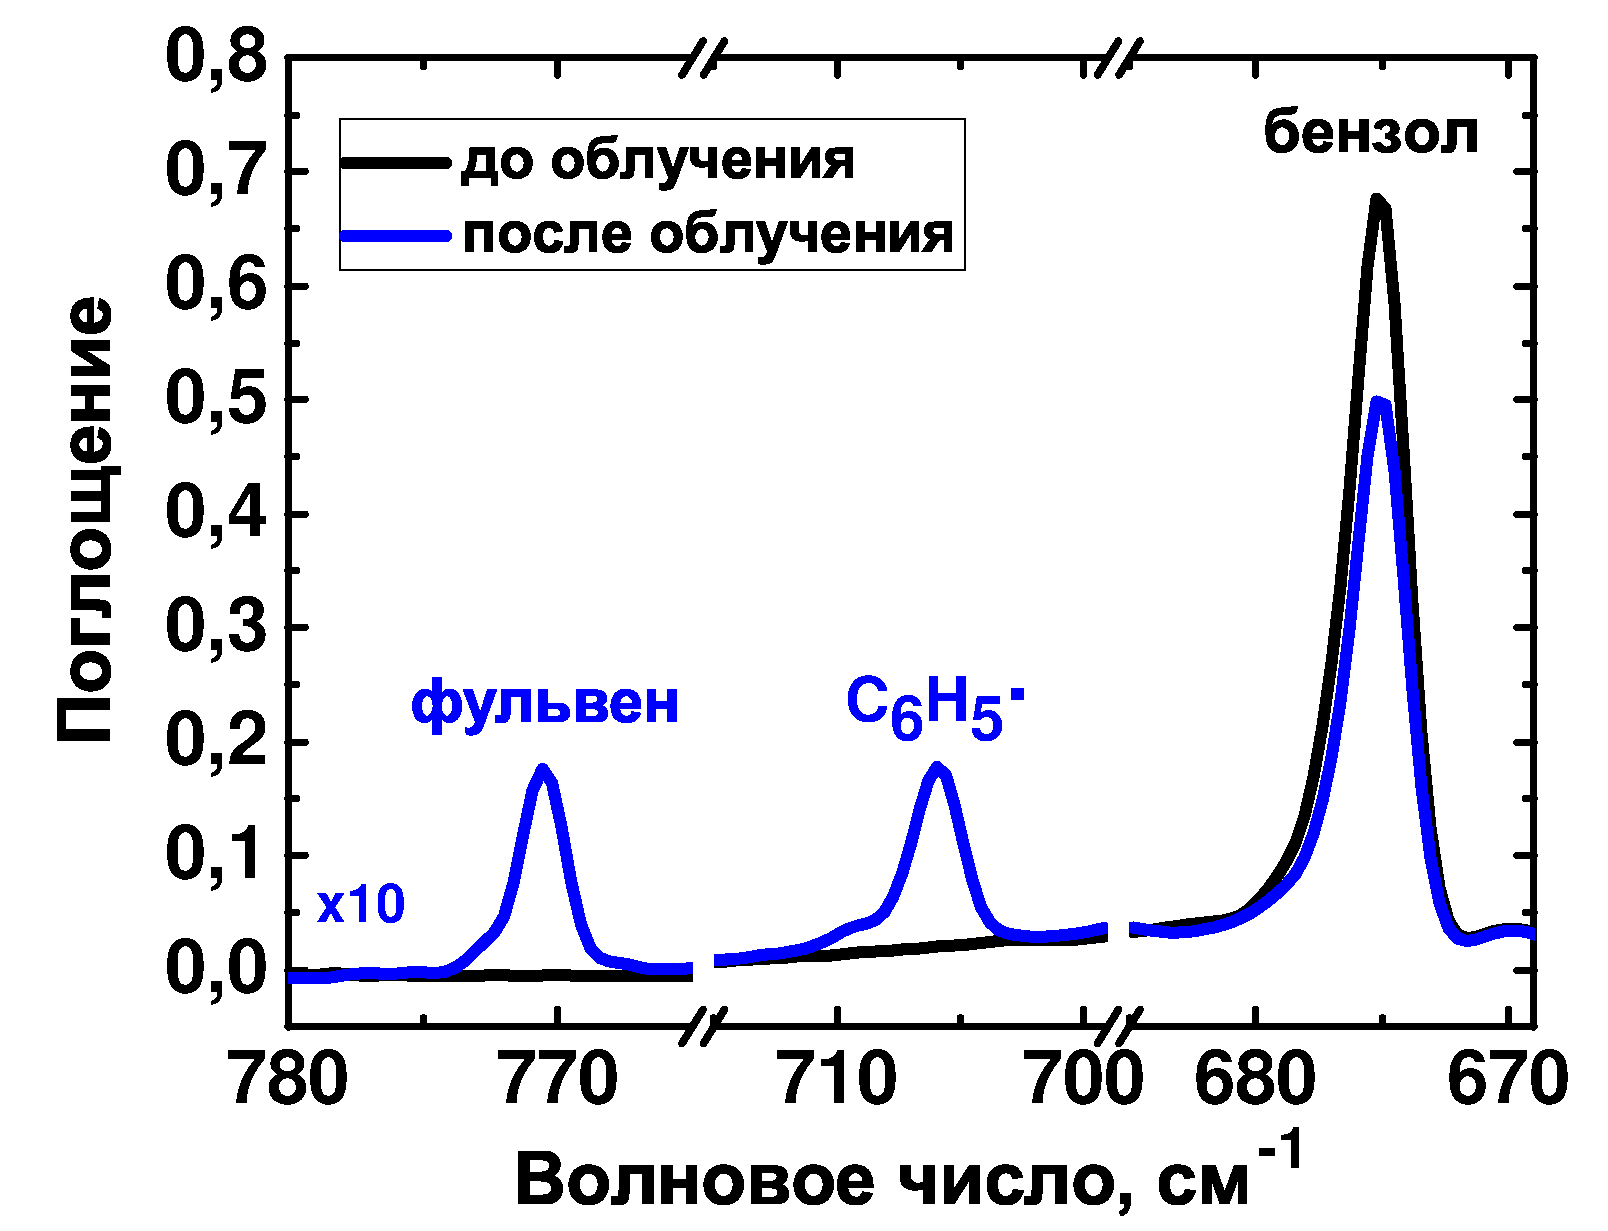
\includegraphics[width=0.5\linewidth]{Ar_sp_irr.pdf} \label{Ar_sp}}  
\subfigure[]{
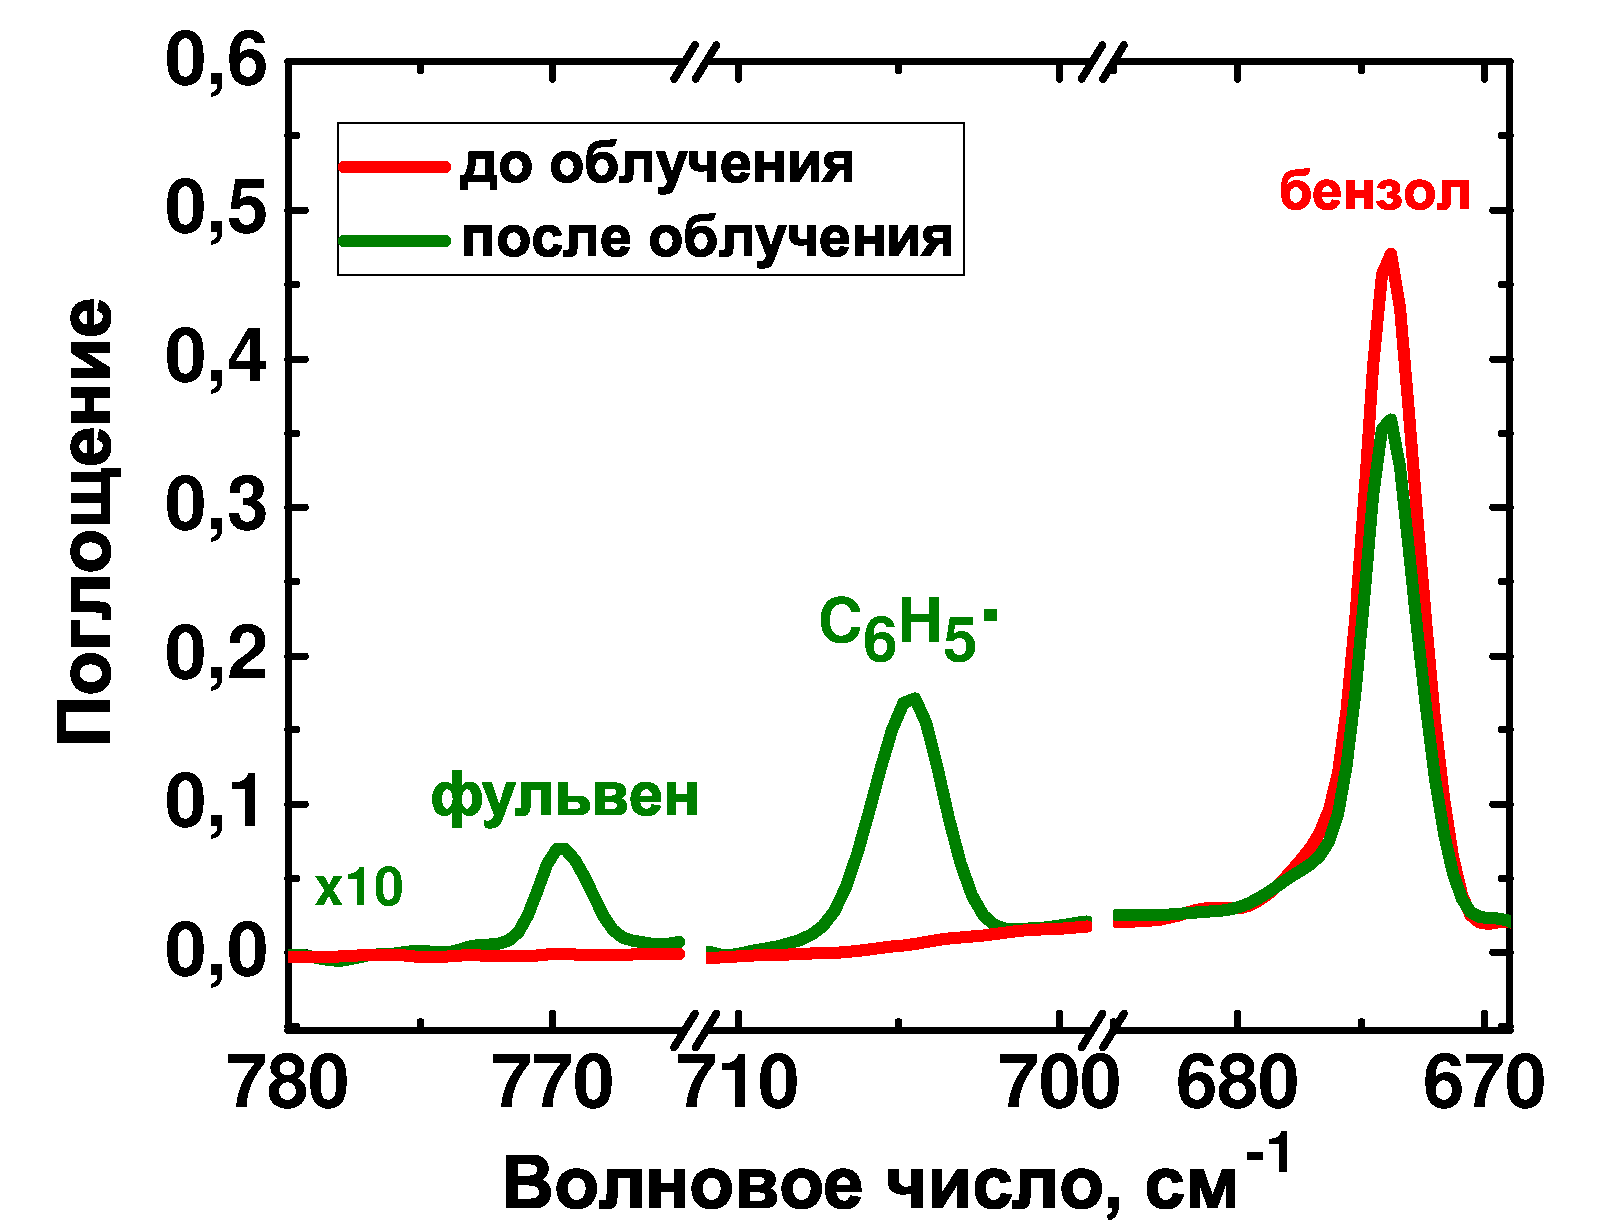
\includegraphics[width=0.5\linewidth]{Kr_sp_irr.pdf} \label{Kr_sp}}
\caption{Фрагменты ИК-спектров бензола в матрицах \subref{Ar_sp}~аргона; \subref{Kr_sp}~криптона до и после облучения} 
\label{spectra}
\end{figure}

\begin{table}[H]
\caption{Волновые числа колебаний фенильного радикала~(см$^{-1}$) в~различных матрицах}
\label{tabl:phenyl}
\begin{center}
\begin{tabular}{ccc}
Ar & Kr & Xe \\
\hline
604.7 & 603.0 & 601.2 \\
657.5 & 656.0 & 654.9 \\
706.0 & 704.8 & 703.9 \\
1026.5 & 1024.8 & 1022.5 \\
1432.2 & 1430.3 & 1429.1 \\
1441.2 & 1439.7 & 1437.9 \\
3087.0 & 3063.8 & 3055.7 \\
\end{tabular}
\end{center}
\end{table}

\begin{table}[H]
\caption{Волновые числа колебаний фульвена~(см$^{-1}$) в~различных матрицах}
\label{fulvene}
\begin{center}
\begin{tabular}{ccc}
Ar & Kr & Xe \\
\hline
616.1 & 615.4 & 614.8 \\
770.6 & 769.7 & 768.6 \\
894.4 & 893.3 & - \\
926.3 & 925.2 & 924.5 \\
1080.9 & - & - \\
1343.0 & 1341.0 & 1339.3 \\
1489.1 & - & - \\
\end{tabular}
\end{center}
\end{table}

Кривые накопления фульвена и фенильного радикала в различных матрицах представлены на рисунке~\ref{tio}. Использовали координаты относительная концентрация продукта -- конверсия бензола (доля разложившегося бензола).
Для получения относительных концентраций каждую интегральную интенсивность сигнала
нормировали на соответствующий молярный коэффициент поглощения, считая, что коэффициент не зависит от матрицы (56~км/моль для внеплоскостных C--H  колебаний фенильного радикала 
(706.0~см$^{-1}$ в~аргоне) по данным эксперимента~\cite{Friderichsen2001}, 50~км/моль  для внеплоскостных C--H колебаний фульвена (770.6~см$^{-1}$ в~аргоне) по данным квантово-химического расчёта без учёта окружения~\cite{Toh2015}). Полученные значения нормировали на максимальную концентрацию фенильного радикала, что необходимо для сравнения данных, которые получены в различных экспериментах в различных матрицах.

Из рисунка~\ref{tio} видно, что в матрицах аргона и криптона оба рассматриваемых продукта появляются сразу после облучения и при малых конверсиях бензола (до 0.1--0.15) накапливаются линейно, а значит они являются первичными.
В матрице ксенона распад бензола на фенильный радикал и атом водорода является доминирующим каналом радиолиза, 
что согласуется с литературными данными (см. раздел~\ref{rad}).
\\
\begin{figure}[H]  
\vspace{-4ex} \centering \subfigure[]{
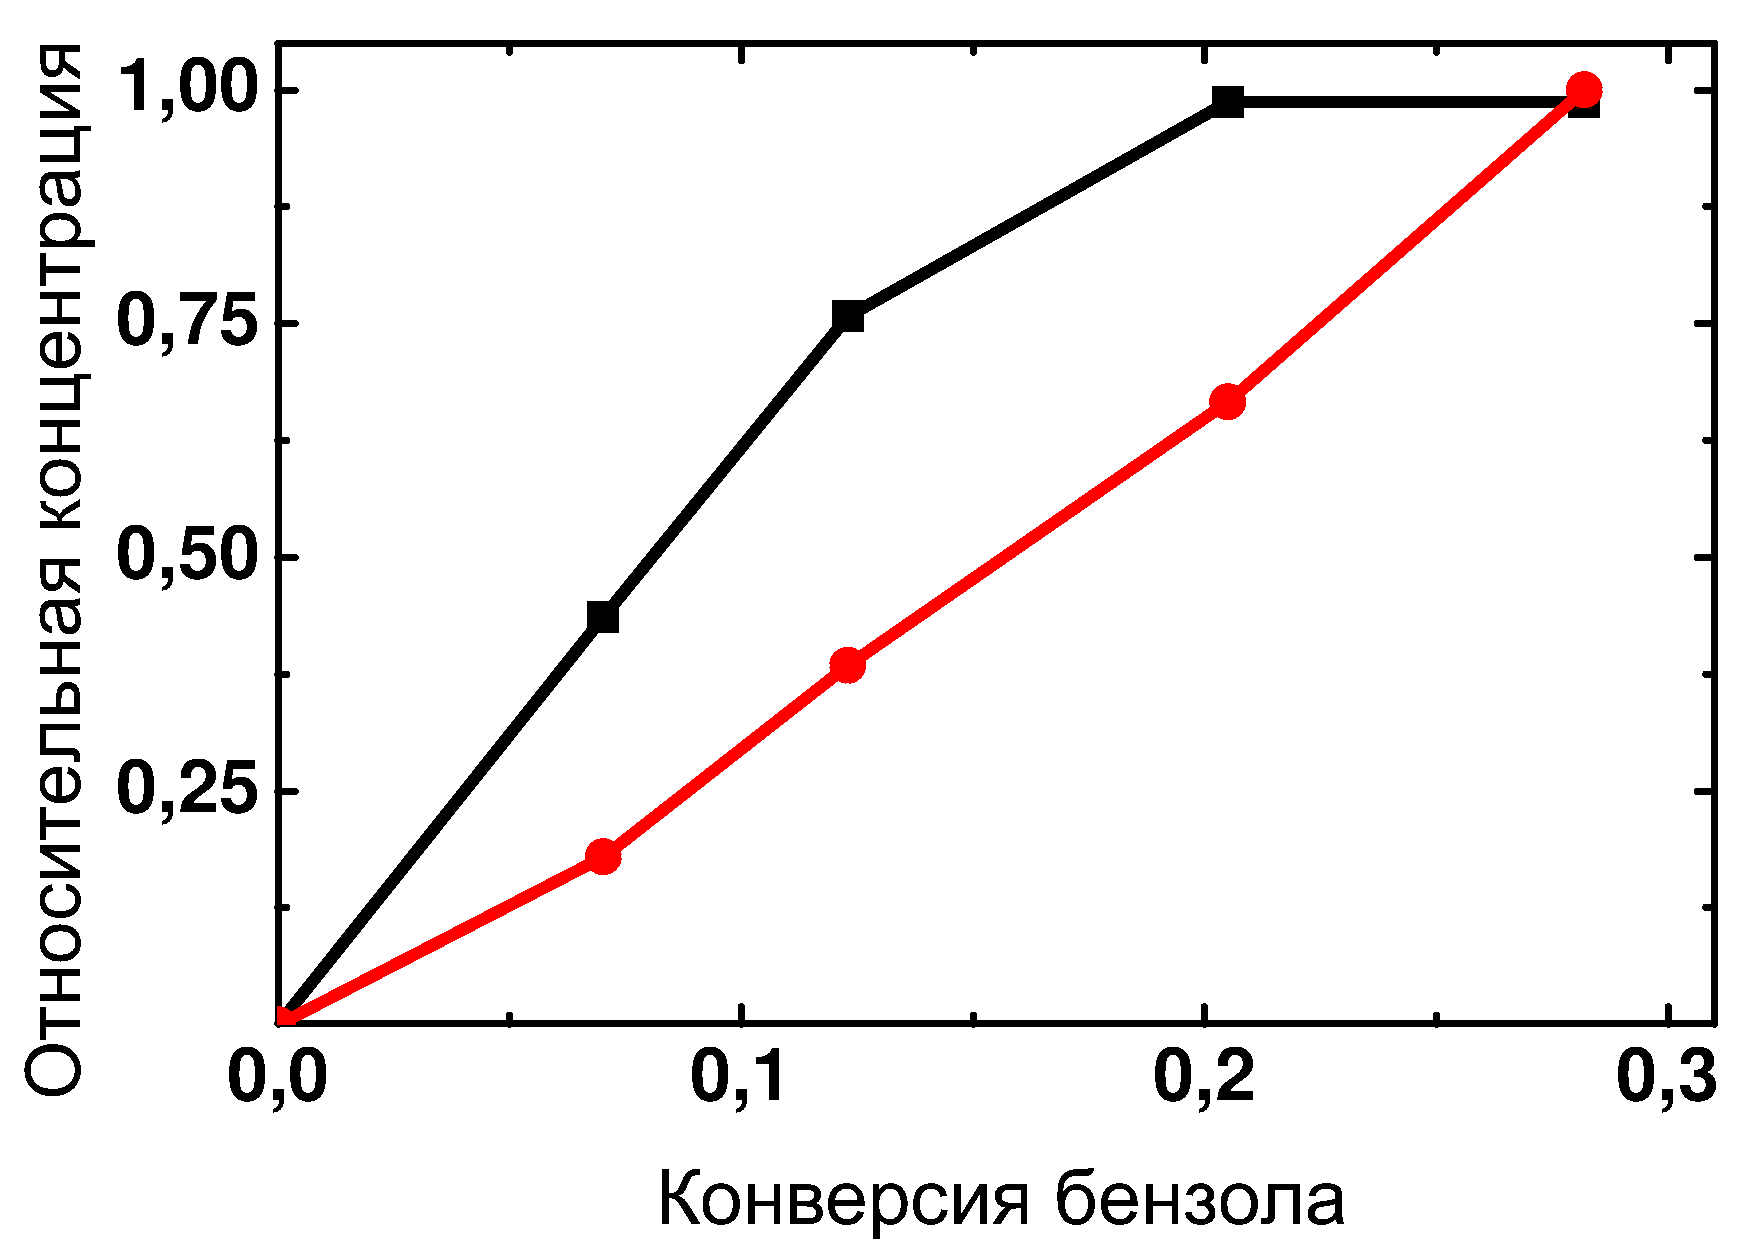
\includegraphics[width=0.6\linewidth]{prodAr+.pdf} \label{prodAr}}  
\hspace{4ex}
\subfigure[]{
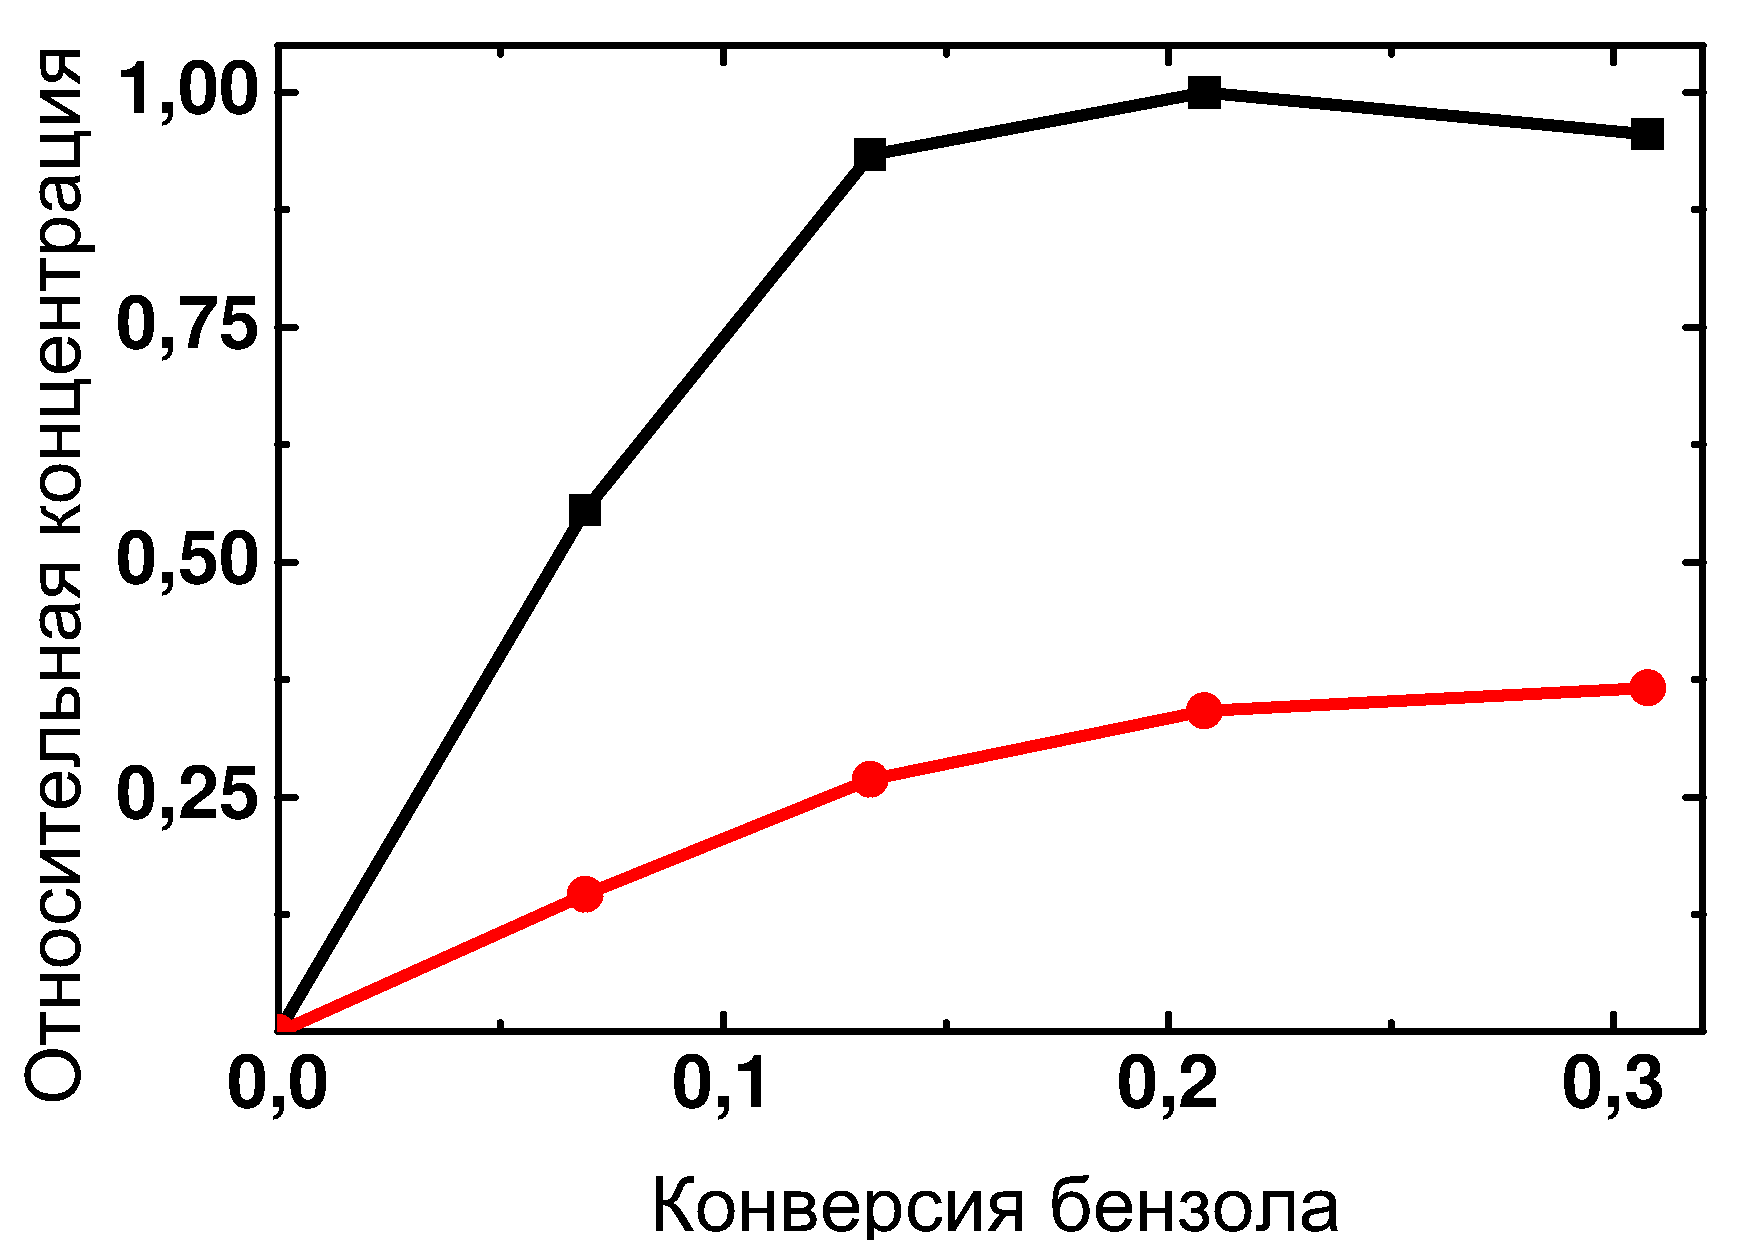
\includegraphics[width=0.6\linewidth]{prodKr+.pdf} \label{prodKr}}
\hspace{4ex}
\subfigure[]{
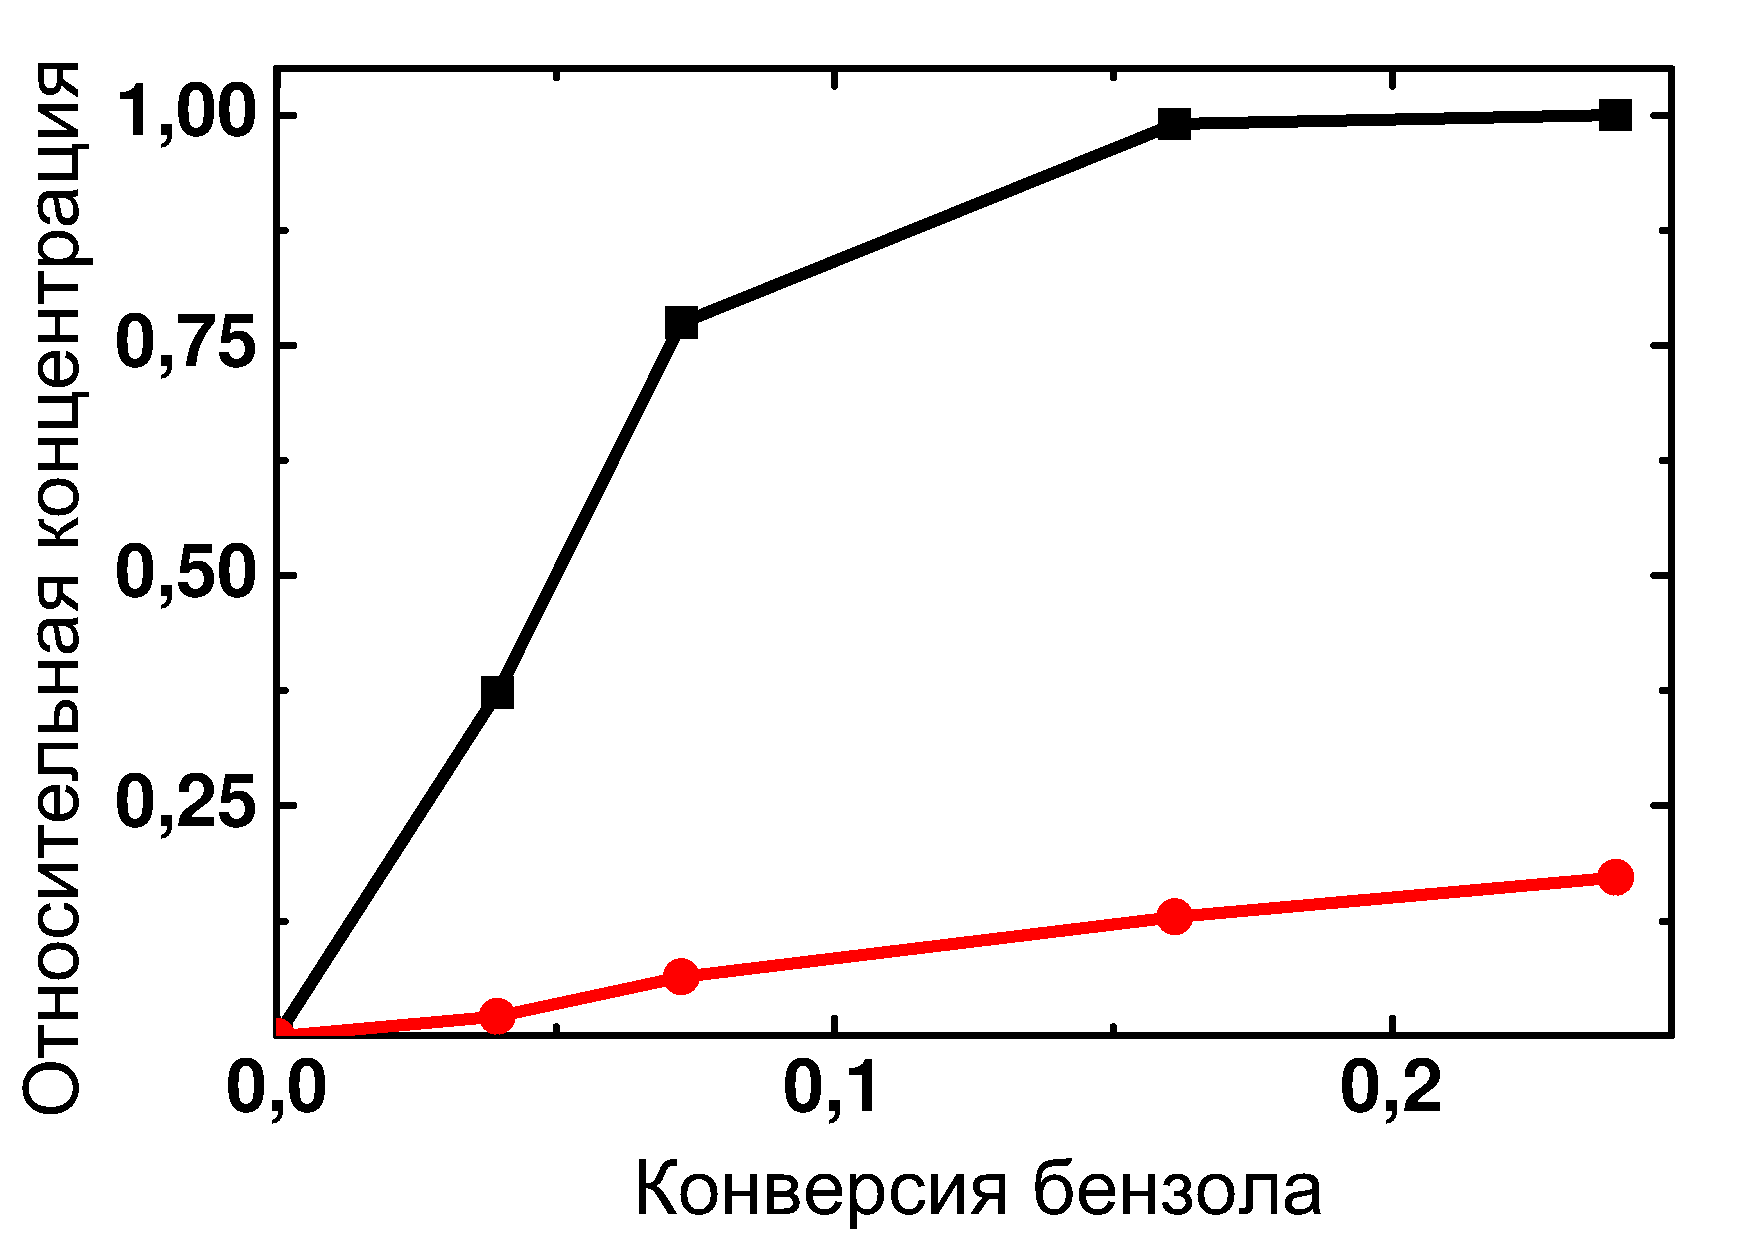
\includegraphics[width=0.6\linewidth]{prodXe+.pdf} \label{prodXe}}  
\caption{Кривые накопления фенильного радикала (чёрный) и фульвена (красный) в матрицах \subref{prodAr} аргона; \subref{prodKr} криптона; \subref{prodXe} ксенона} \label{tio}
\end{figure}
\newpage
Полученные из кривых накопления фенильного радикала и фульвена (рисунок~\ref{tio}) отношения концентраций (а значит, и отношения радиационно-химических выходов) фенильного радикала и фульвена представлены на рисунке \ref{rel}.  Это отношение сильно увеличивается при переходе от матриц аргона и криптона к матрице ксенона.
 
 \begin{figure}[h!]
\center{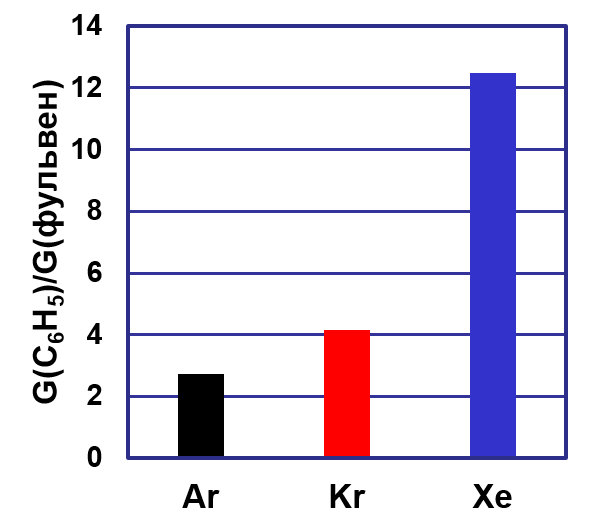
\includegraphics[width=0.5\linewidth]{rel1.png}}
\caption{Отношение выходов фенильного радикала и фульвена в различных матрицах}
\label{rel}
\end{figure}

Рост отношения выходов фенильного радикала и фульвена при переходе от матрицы аргона к матрице ксенона может быть связан как с увеличением выхода фенильного радикала, так и с уменьшением выхода фульвена в ряду Ar--Kr--Xe. Уменьшение радиационно-химического выхода фульвена в ряду Ar>Kr>Xe может быть объяснено увеличением эффективности интеркомбинационной конверсии. При переходе от матрицы аргона к матрице ксенона
понижается выход синглетных возбуждённых состояний бензола, из которых и образуется фульвен (см. раздел~\ref{photolysis}). Фенильный радикал образуется предположительно из высших триплетных возбуждённых состояний бензола. Эффективная интеркомбинационная конверсия повышает выход триплетных состояний бензола в матрицах криптона и ксенона, а значит радиационно-химический выход радикала C$_6$H$_5^\bullet$ должен расти в ряду Ar<Kr<Xe. Таким образом, увеличение выхода фенильного радикала и понижение выхода фульвена приводит к наблюдаемому изменению отношения их концентраций. 

Кроме того, необходимо отметить, что при рекомбинации возникающих при радиолизе электронов и катион-радикалов бензола образуются высшие триплетные и синглетные состояния бензола в отношении 3:1.  Этим обусловлено эффективное образование C$_6$H$_5^\bullet$ радикала при радиолизе бензола и его отсутствие при фотолизе, когда  высшие триплетные состояния практически не заселяются (см. разделы~\ref{radiolysis}, \ref{photolysis}). 


В ИК-спектрах облучённых образцов C$_6$H$_6$/Ng (Ng~= Ar, Kr, Xe) наблюдаются радиационно-индуцированные полосы поглощения в области 3330~см$^{-1}$ (см. рисунок~\ref{135_}), демонстрирующие ускорение роста с увеличением конверсии бензола (см. рисунок~\ref{135r}, каждая кривая пронормирована на собственное максимальное значение для возможности сравнения данных, полученных в различных матрицах). Такое поведение типично для продуктов вторичных радиационно-индуцированных реакций. Можно сделать предположение, что наборы полос, приведённые в таблицах~\ref{135}, \ref{1351}, соответствуют {\it цис}- и {\it транс}-изомерам гексадиен\nobreakdash-1,3\nobreakdash-ина\nobreakdash-5, так как образование данных продуктов описано при радиолизе и фотолизе бензола (см. раздел~\ref{radiolysis},~\ref{photolysis}). Кроме того, экспериментально полученные волновые числа удовлетворительно согласуются с данными квантово-химических расчётов. Многие полосы поглощения имеют сложную подструктуру, обусловленную наличием различных конформеров гексадиен\nobreakdash-1,3\nobreakdash-ина\nobreakdash-5, а так же <<сайтовым>> расщеплением (см. раздел \ref{isolation}).

 \begin{figure}[H]
\center{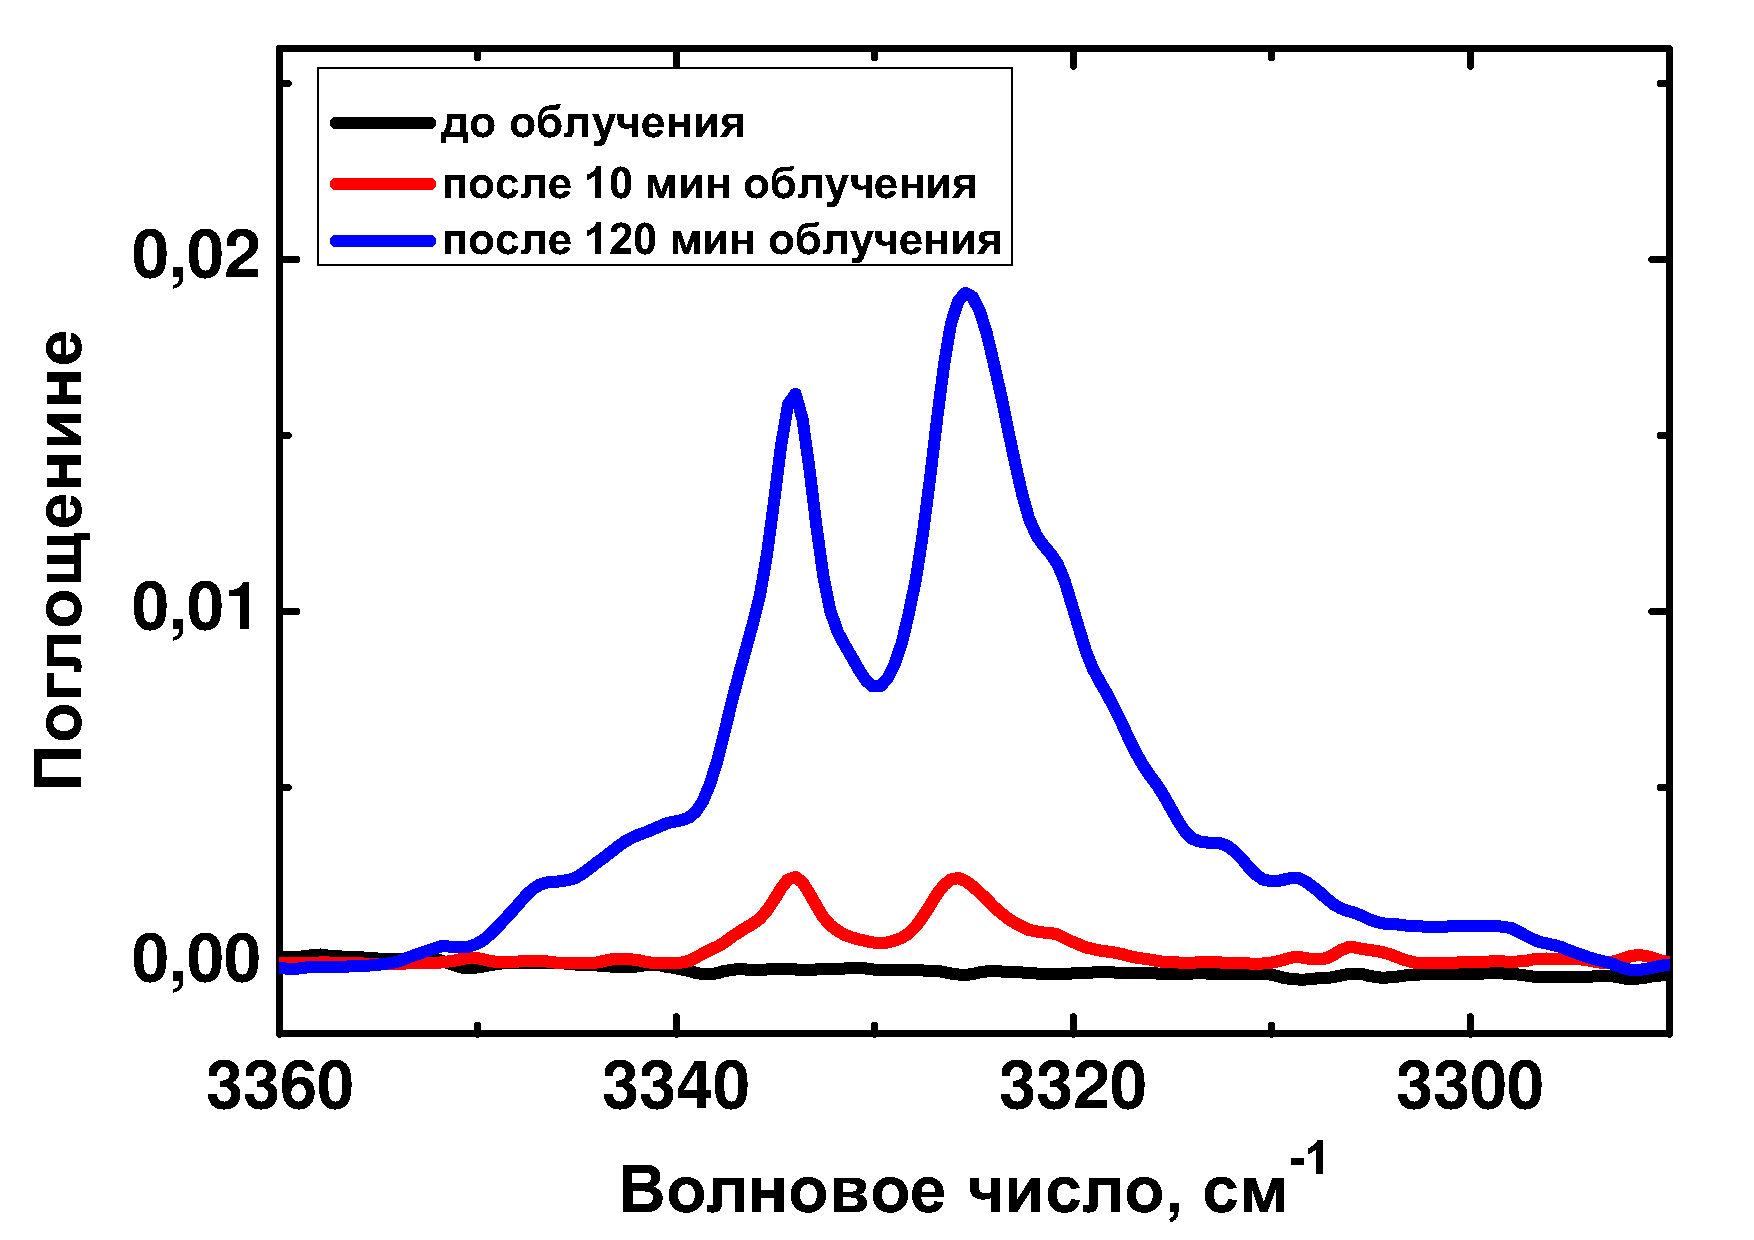
\includegraphics[width=0.9\linewidth]{135_.pdf}}
\caption{Фрагменты ИК-спектров образца C$_6$H$_6$/Ar, содержащие полосы поглощения гексадиен\nobreakdash-1,3\nobreakdash-ина\nobreakdash-5}
\label{135_}
\end{figure}

 \begin{figure}[H]
\center{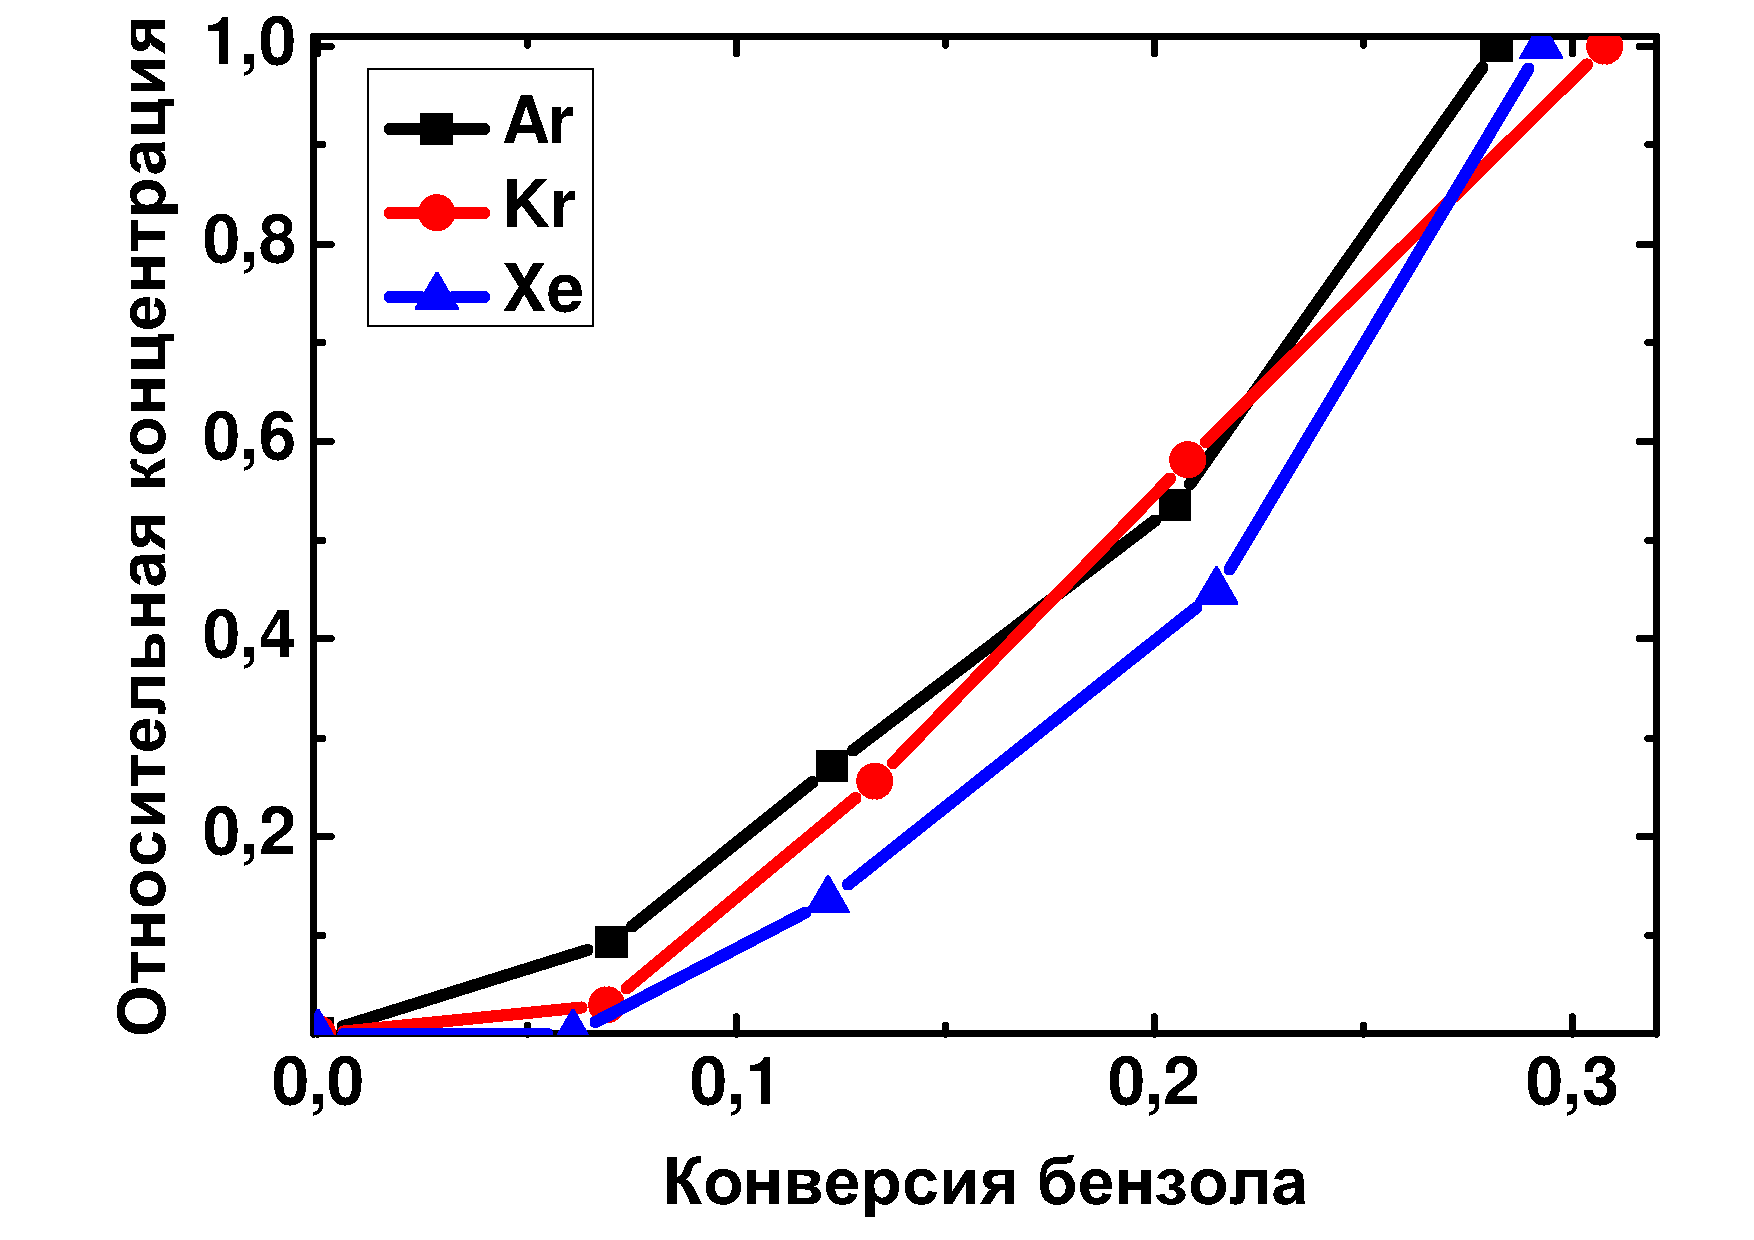
\includegraphics[width=0.9\linewidth]{135_s.pdf}}
\caption{Кривые накопления гексадиен\nobreakdash-1,3\nobreakdash-ина\nobreakdash-5 в различных матрицах}
\label{135r}
\end{figure}

\begin{table}[H]
\caption{Экспериментальные волновые числа~(Ar, Kr, Xe) и расчётные частоты~(PBE/L2\_3) колебаний {\it цис}-гексадиен\nobreakdash-1,3-ина-5~(см$^{-1}$)}
\label{135}
\begin{center}
\begin{tabular}{cccc}
Ar & Kr & Xe & Расчёт \\
\hline
620.9 & 619.7 & - & 620.8\\
759.2 & 758.7 & - & 765.2\\
913.5 & 912.6 & 909.8 & 910.2\\
1000.9 & 998.6 & 997.2 & 1001.68\\
1004.2 & 1002.6 & 1000.2 & 1006.78\\
3334.0 & 3333.9 & 3326.2 & 3407.3\\
3336.9 &  & \\
\end{tabular}
\end{center}
\end{table}

\begin{table}[H]
\caption{Экспериментальные волновые числа~(Ar, Kr, Xe) и расчётные частоты~(PBE/L2\_3) колебаний {\it транс}-гексадиен\nobreakdash-1,3-ина-5~(см$^{-1}$)}
\label{1351}
\begin{center}
\begin{tabular}{cccc}
Ar & Kr & Xe & Расчёт \\
\hline
630.9 & 629.8 & 626.4 & 629.3\\
894.3 & 893.3 & 892.1 & 897.1\\
948.7 & 947.1 & 946.1 & 946.9\\
3325.7 & 3313.4 & 3315.2 & 3408.9\\
 & 3325.9 & 3312.4 & \\
\end{tabular}
\end{center}
\end{table}

Известно, что гексадиен\nobreakdash-1,3\nobreakdash-ин\nobreakdash-5 может образовываться из фульвена при фотолизе. В матрицах криптона и ксенона при конверсиях бензола больше 0.15 образование фульвена замедляется, следовательно, логично предположить, что и в данном случае гексадиен\nobreakdash-1,3\nobreakdash-ин\nobreakdash-5 образуется из фульвена. В матрице аргона кривая накопления фульвена практически линейна, при этом некоторые количества гексадиен\nobreakdash-1,3\nobreakdash-ина\nobreakdash-5 образуются уже при малых конверсиях бензола. Это свидетельствует о наличии альтернативного <<одностадийного>> механизма образования гексадиен\nobreakdash-1,3\nobreakdash-ина\nobreakdash-5 в матрице аргона. Молекула фульвена, образующаяся в возбуждённом состоянии, не релаксирует в основное состояние, а сразу же претерпевает изомеризацию. Вклад данного механизма наиболее значителен именно в матрице аргона, так как в случае более поляризуемых матриц (Kr, Xe)  релаксация образующегося фульвена протекает значительно эффективнее.
 
Фотолиз облучённых образцов C$_6$H$_6$/Ng в видимой области и ближнем УФ-диапазоне не приводит к значительным изменениям в ИК-спектре ни в одной из матриц. 

\subsection{Радиолиз бензола-$d_6$}

В ИК-спектрах осаждённых образцов C$_6$D$_6$/Ng присутствуют полосы поглощения, соответствующие дейтерированному бензолу. Отнесение основано на литературных спектроскопических данных для газовой фазы с учётом разумных матричных сдвигов~\cite{Shimanouchi}. 
Типичный вид спектра осаждённой смеси представлен на рисунке~\ref{Ar_d6}. 

 \begin{figure}[H]
\center{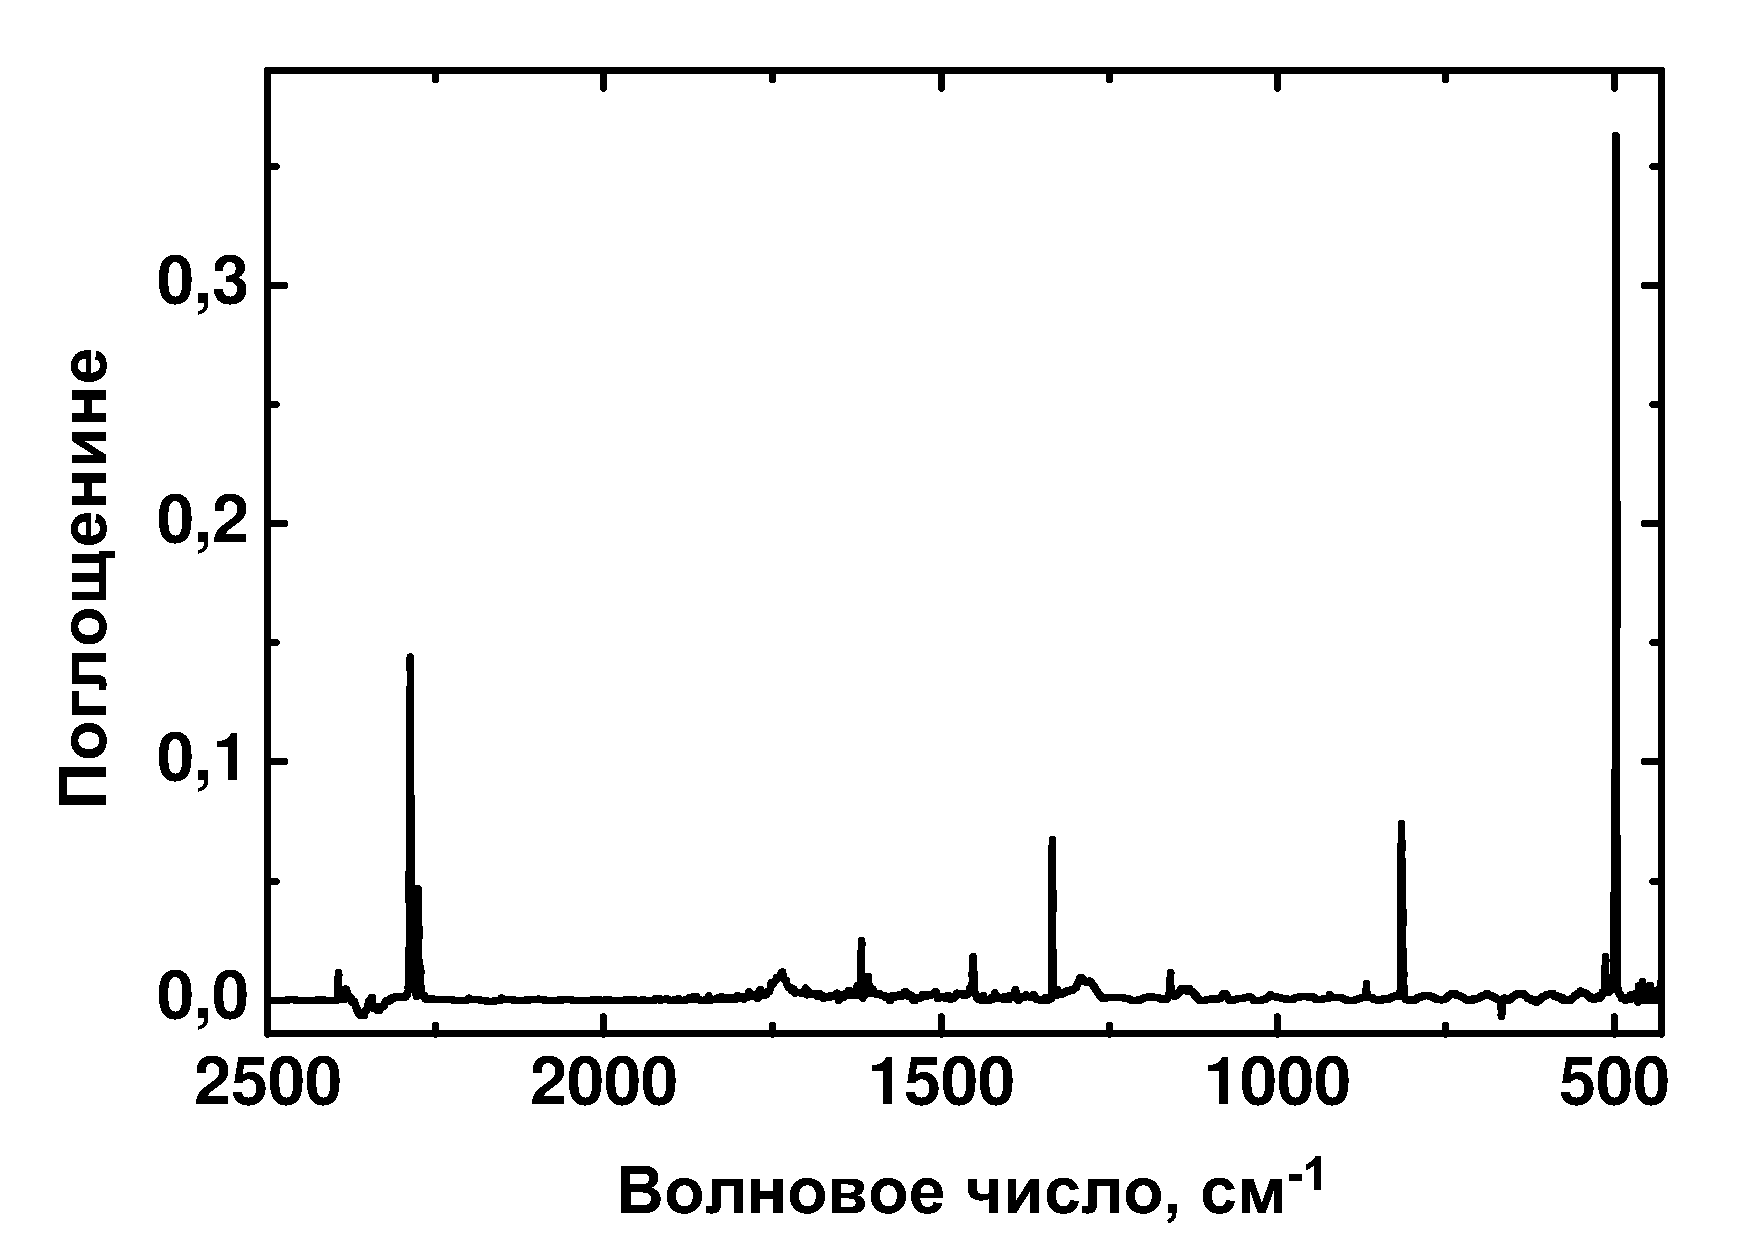
\includegraphics[width=0.9\linewidth]{is_d.pdf}}
\caption{ИК-спектр осаждённой смеси C$_6$D$_6$/Ar 1:1000}
\label{Ar_d6}
\end{figure}


В результате радиолиза осаждённых образцов C$_6$D$_6$/Ng (Ng~= Ar, Kr, Xe) дейтерированный бензол разлагается довольно эффективно. На рисунке~\ref{comp} представлены кривые расходования C$_6$D$_6$ в различных матрицах, для сравнения приведены кривые расходования C$_6$H$_6$. Из данных зависимостей видно, что бензол\nobreakdash-$d_6$ расходуется немного медленнее, чем недейтерированный бензол в соответствующих матрицах. Закономерно, что радиационно-химические выходы расходования бензола-$d_6$, определённые из начальных участков кривых аналогично случаю недейтерированного бензола по уравнению \ref{yee}, составили: для матрицы аргона $G$(--C$_6$D$_6$)~= 1.5~молек./100~эВ, для матриц криптона и ксенона    $G$(--C$_6$D$_6$)~= 0.3~молек./100~эВ.


 \begin{figure}[H]
\center{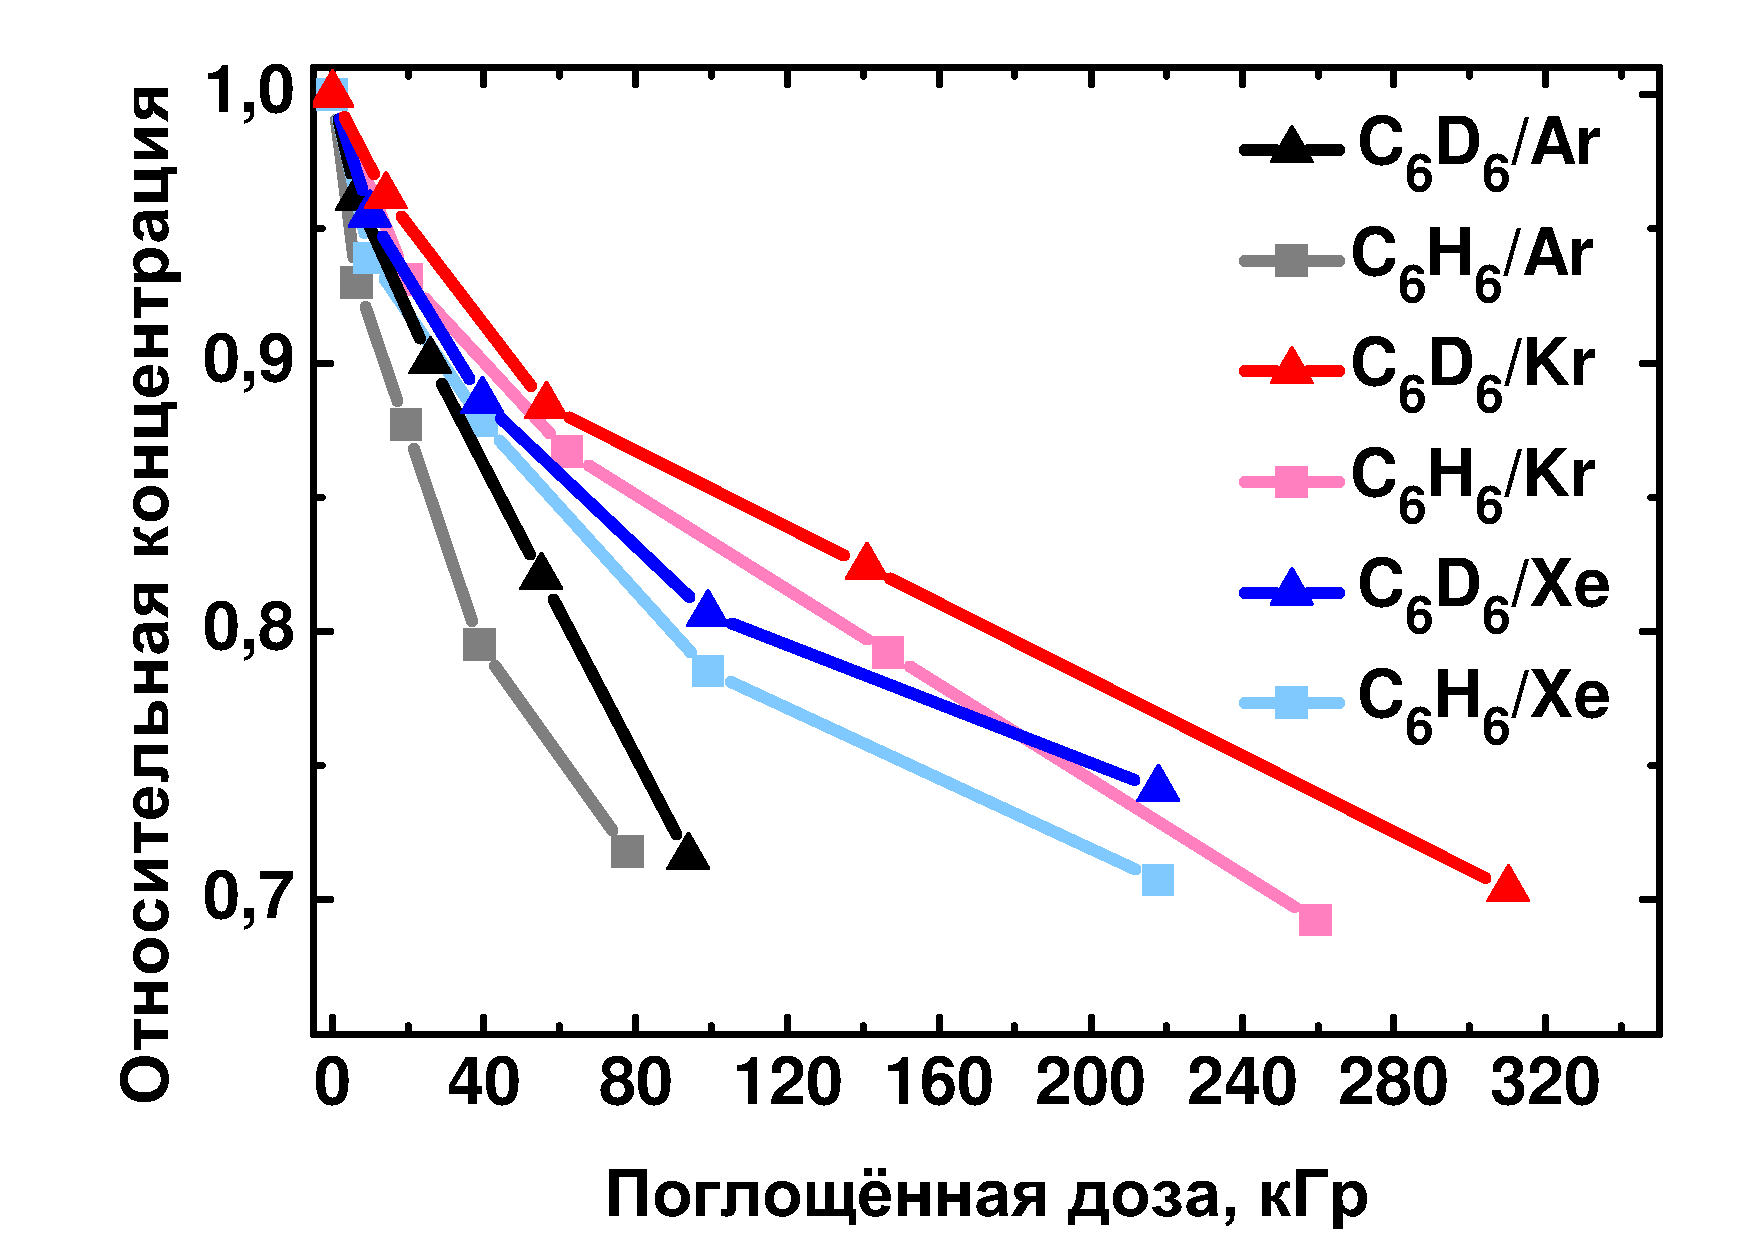
\includegraphics[width=0.9\linewidth]{comp_dose_2col.pdf}}
\caption{Зависимости относительной концентрации бензола и бензола-$d_6$ от поглощённой дозы}
\label{comp}
\end{figure}

После облучения образцов C$_6$D$_6$/Ng в ИК-спектрах появляются дополнительные полосы поглощения. Во всех матрицах наблюдается образование радикала~C$_6$D$_5^\bullet$ (см. таблицу~\ref{C6D5}), отнесение основано на литературных данных~\cite{Friderichsen2001}. Спектроскопические характеристики фульвена-$d_6$ в литературе отсутствуют, однако логично предположить образование фульвена-$d_6$ при радиолизе смесей C$_6$D$_6$/Ng, аналогично экспериментам с образцами С$_6$Н$_6$/Ng. Действительно, волновые числа радиационно-индуцированных полос поглощения хорошо согласуются с данными квантово-химических расчётов (см. таблицу~\ref{fd6}).

 \begin{table}[H]
\caption{Волновые числа колебаний радикала C$_6$D$_5^\bullet$~(см$^{-1}$) в~различных матрицах}
\label{C6D5}
\begin{center}
\begin{tabular}{ccc}
Ar & Kr & Xe \\
\hline
517.7 & 517.2 & 516.1 \\
- & - & 587.8 \\
802.8 & 801.2 & 799.9 \\
806.0 & 804.5 & 802.7 \\
- & - & 1308.8 \\
- & 1312.6 & 1311.9 \\
\end{tabular}
\end{center}
\end{table}


 \begin{table}[H]
\caption{Экспериментальные волновые числа~(Ar, Kr, Xe) и расчётные частоты~(PBE/L2\_3) колебаний фульвена-$d_6$~(см$^{-1}$)}
\label{fd6}
\begin{center}
\begin{tabular}{cccc}
Ar & Kr & Xe & Расчёт\\
\hline
487.8 & 487.2 & 486.7 & 484.6\\
489.2 & 488.9 & 488.2 & \\
773.1 & 772.0 & 771.1 & 777.2 \\
1447.0 & - & - & 1455.4\\
\end{tabular}
\end{center}
\end{table}

Кривые накопления основных продуктов радиолиза бензола-$d_6$ в различных матрицах представлены на рисунке \ref{tio-d}. Для их получения использованы следующие молярные коэффициенты поглощения: 18.7~км/моль для полосы поглощения, соответствующей внеплоскостным колебаниям в группе CD$_2$ фульвена (773.1~см$^{-1}$ в аргоне), 29.3~км/моль для полосы поглощения, соответствующей внеплоскостным колебаниям связи C--H фенильного радикала (517.7~см$^{-1}$ в аргоне), оба коэффициента получены в результате квантово-химических расчётов (для C$_6$D$_5^\bullet$ из \cite{Friderichsen2001}). Накопление C$_6$D$_5^\bullet$ и фульвена-$d_6$ протекает, в целом, аналогично случаю недейтерированного бензола, однако в случае C$_6$D$_6$ относительная концентрация фульвена-$d_6$  несколько выше. Начальные участки кривых накопления линейны, поэтому можно сделать вывод о том, что оба продукта являются первичными в матрицах аргона и криптона; в матрице ксенона C$_6$D$_5^\bullet$ также является первичным продуктом, а фульвена образуются только незначительные количества.

\begin{figure}[H]  
\vspace{-4ex} \centering \subfigure[]{
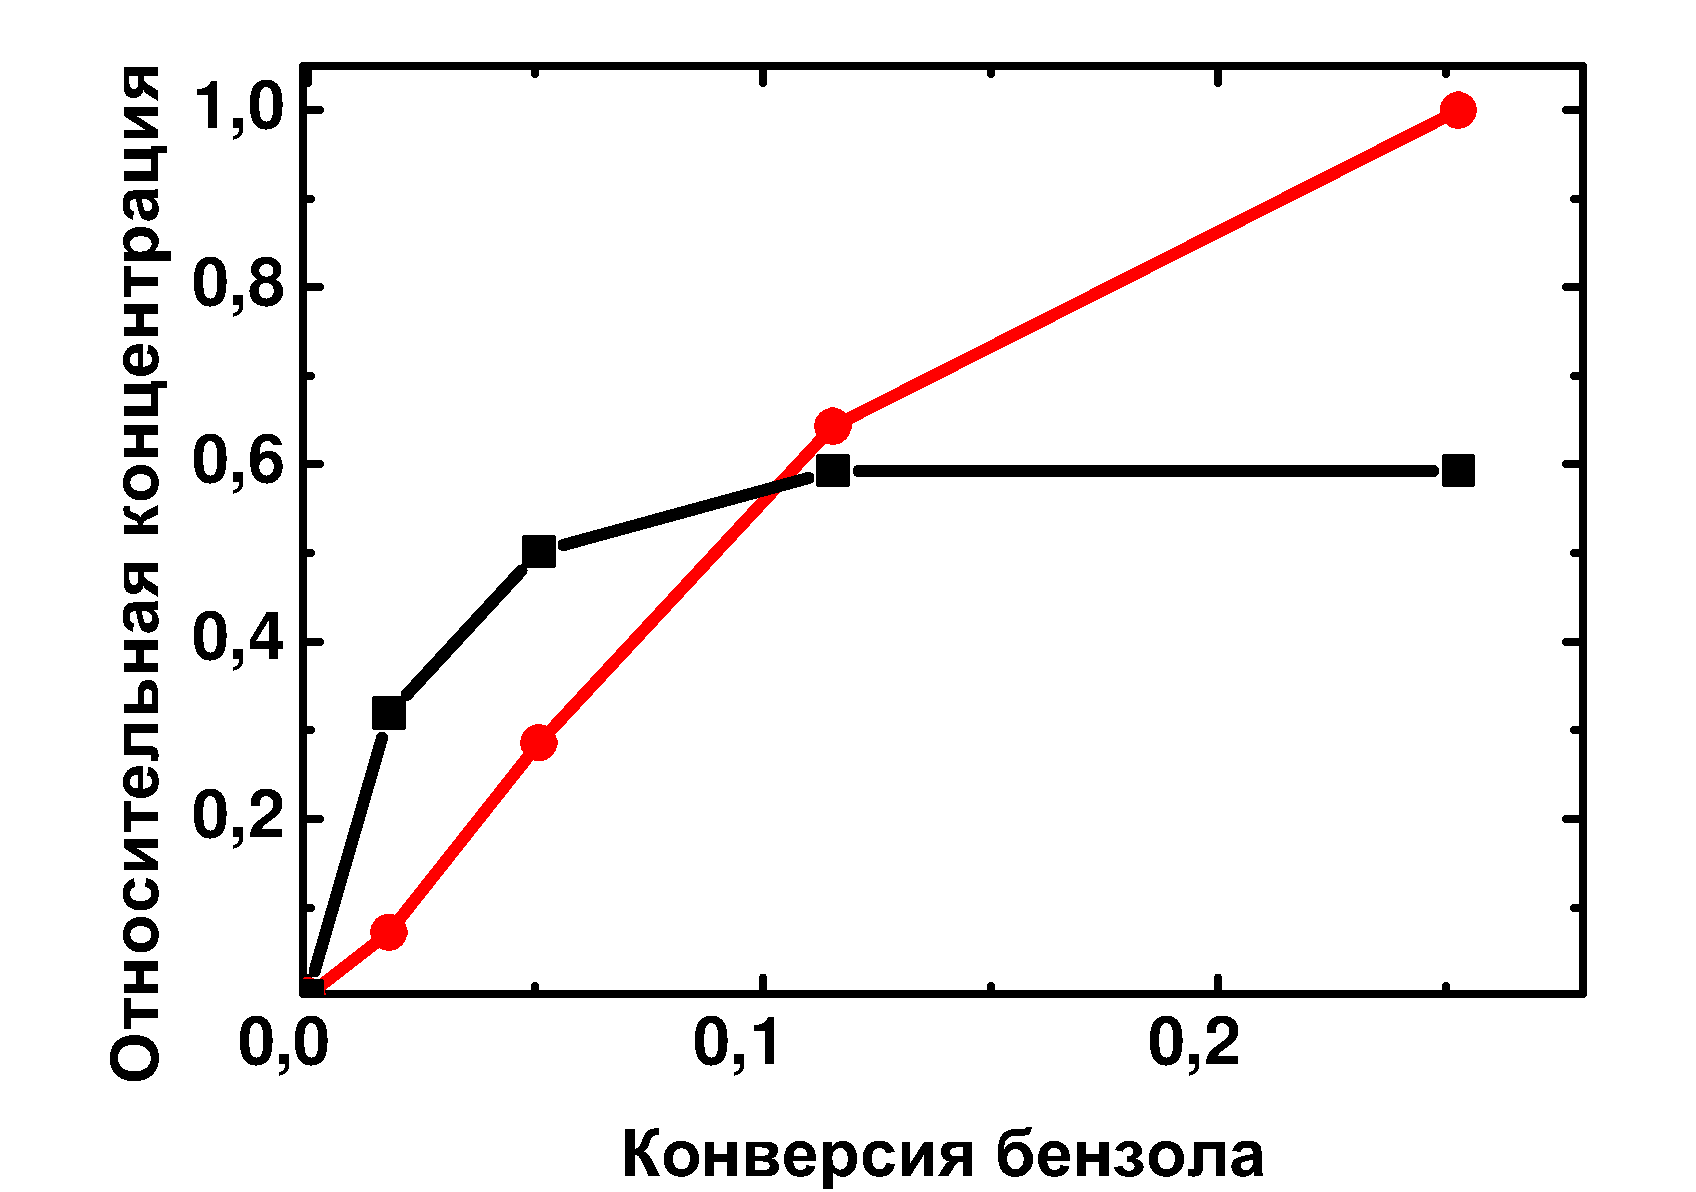
\includegraphics[width=0.6\linewidth]{prod_Ar_d6_xxxx.pdf} \label{prod_Ar_d6}}  
\hspace{4ex}
\subfigure[]{
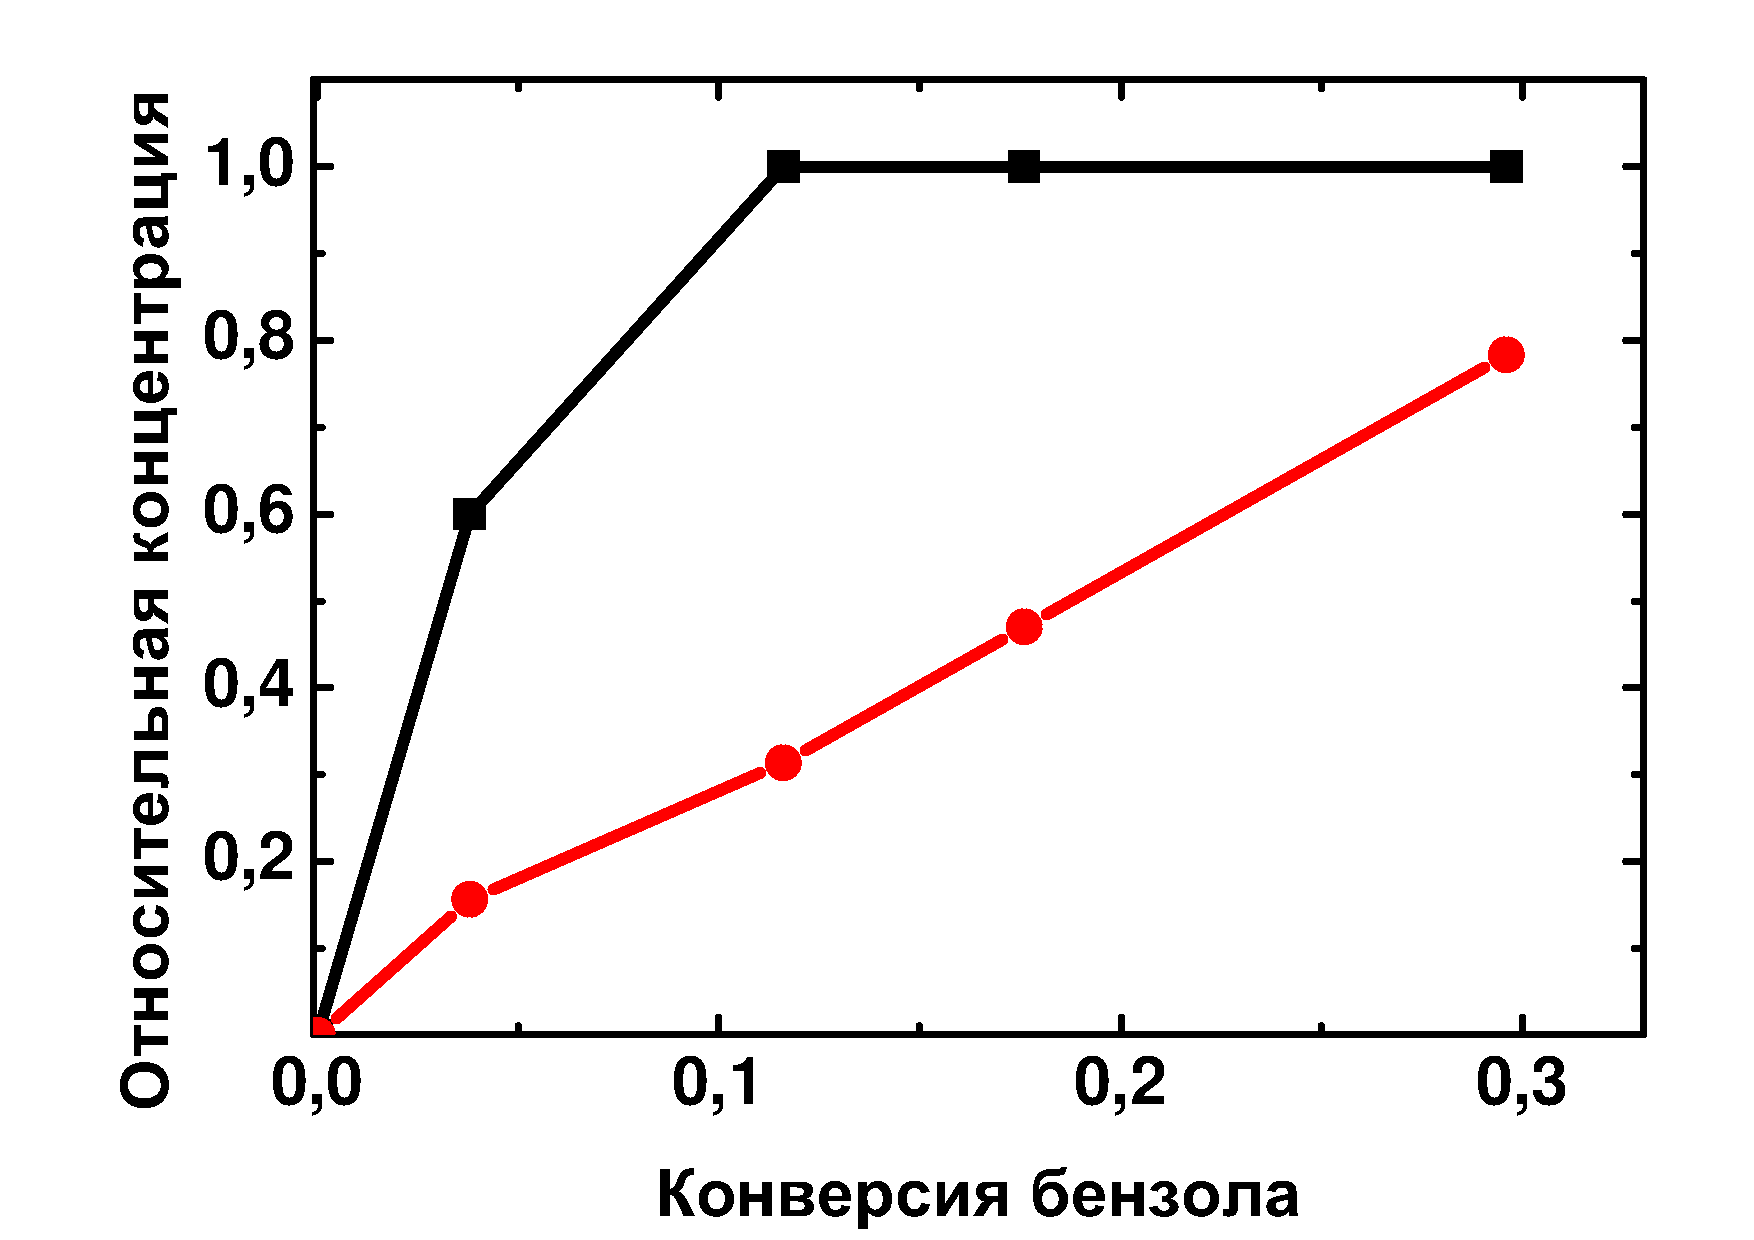
\includegraphics[width=0.6\linewidth]{prod_Kr_d6_xxxx.pdf} \label{prod_Kr_d6}}
\hspace{4ex}
\subfigure[]{
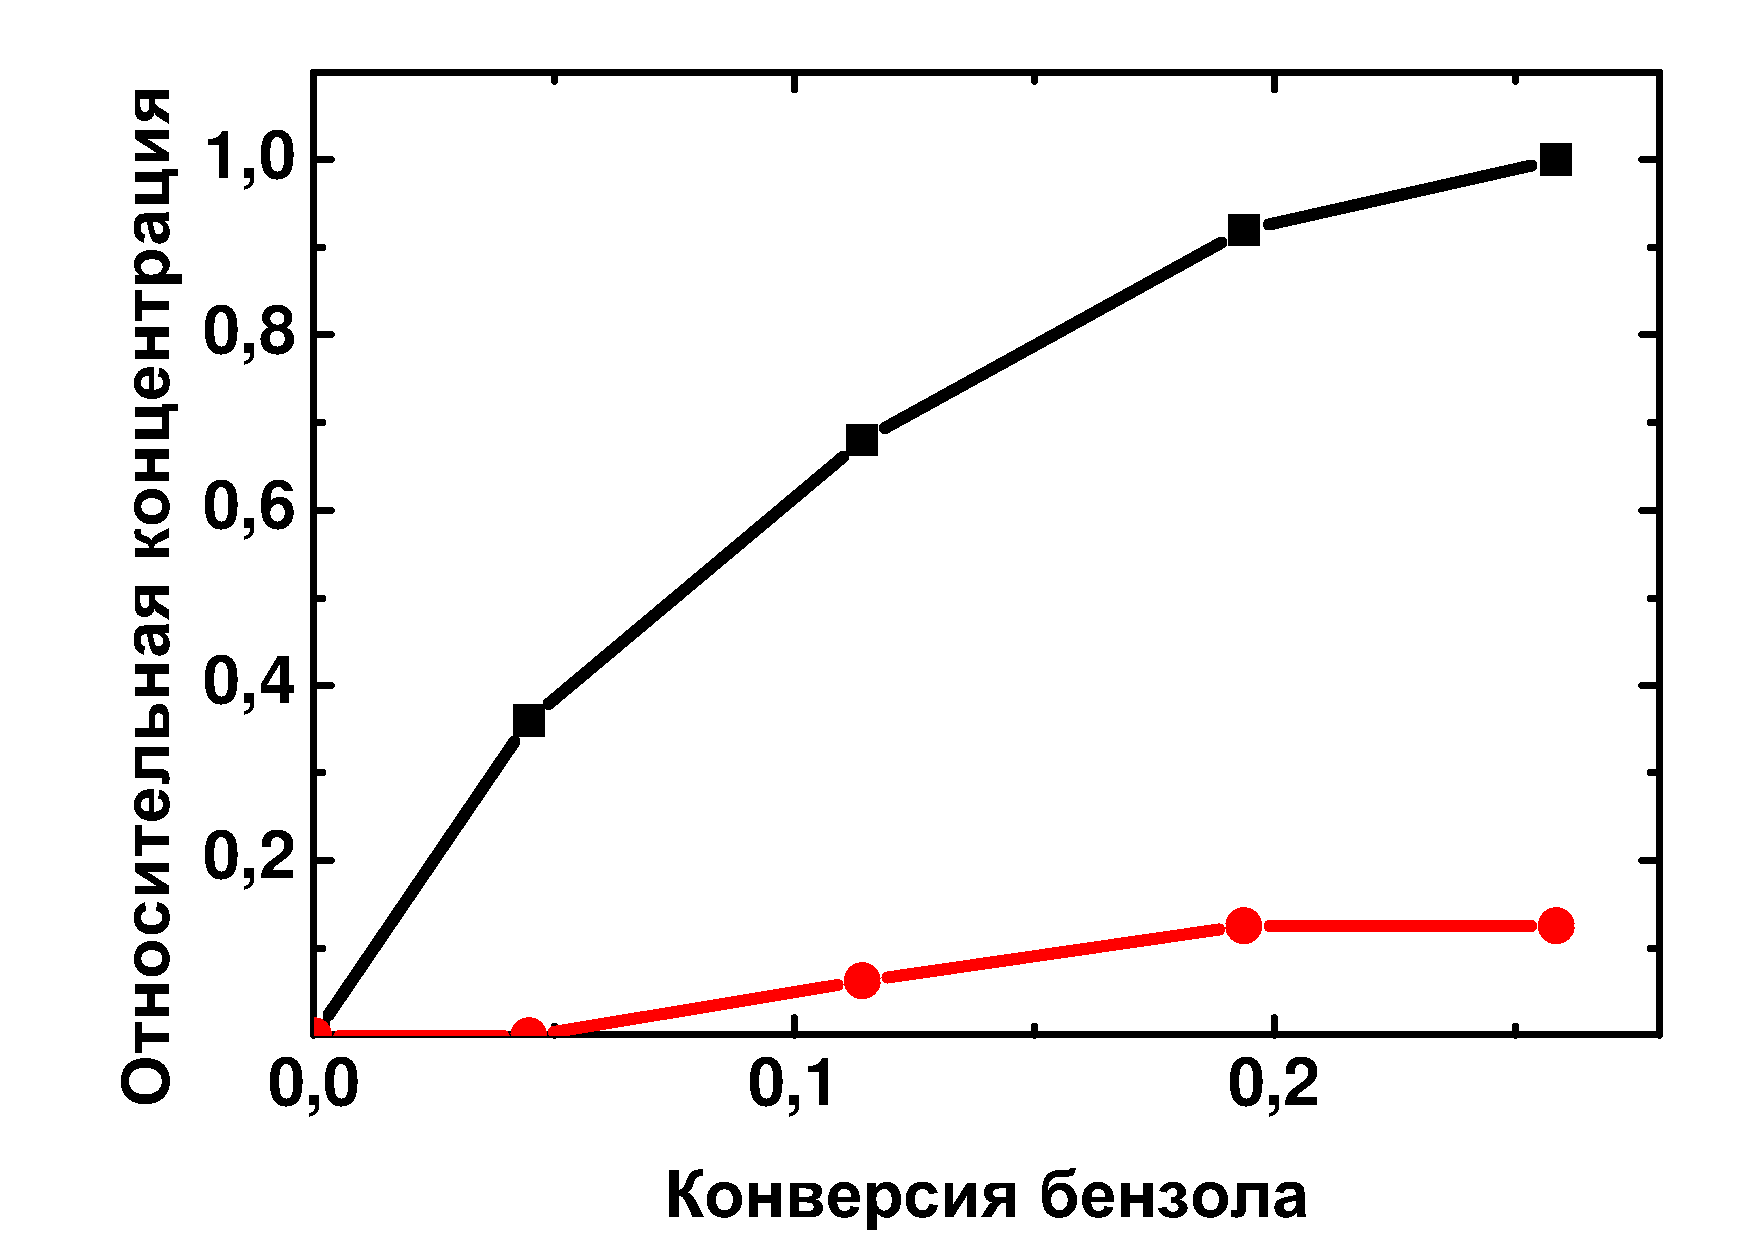
\includegraphics[width=0.6\linewidth]{prod_Xe_d6_xxxx.pdf} \label{prod_Xe_d6}}  
\caption{Кривые накопления фенильного радикала C$_6$D$_5^\bullet$ (чёрный) и фульвена-$d_6$ (красный) в матрицах \subref{prod_Ar_d6}~аргона; \subref{prod_Kr_d6}~криптона; \subref{prod_Xe_d6}~ксенона} \label{tio-d}
\end{figure}

 Отношение интенсивностей радикала C$_6$D$_5^\bullet$ и фульвена-$d_6$ увеличивается в ряду Ar<Kr<Xe. Причины этой закономерности аналогичны случаю недейтерированного бензола.

После облучения бензола-$d_6$ в матрицах аргона и криптона присутствуют полосы поглощения сольватированного дейтрона Ng$_2$D$^+$ (643.2~см$^{-1}$ для Ar и 605.8~см$^{-1}$ для Kr). В случае  ксенона не наблюдается образования значительных количеств Xe$_2$D$^+$. Его полоса поглощения имеет волновое число 517~см$^{-1}$, то есть накладывается на полосу поглощения радикала C$_6$D$_5^\bullet$, однако интенсивность этой полосы при фотолизе в УФ-диапазоне не уменьшается, а значит она соответствует только радикалу, но не  сольватированному дейтрону (см. раздел~\ref{isolation}).

 Во всех матрицах при радиолизе бензола-$d_6$ наблюдается появление интенсивных полос поглощения в области 2600~см$^{-1}$. Данные полосы демонстрируют ускорение роста с увеличением конверсии бензола, что характерно для вторичных продуктов радиационно-индуцированных реакций.  Волновые числа этих полос поглощения примерно в $\sqrt{2}$~ раз меньше, чем волновые числа полос поглощения валентных C--H колебаний при тройной связи гексадиен\nobreakdash-1-ина\nobreakdash-5 (3300~см$^{-1}$).  Можно предположить, что в результате радиационно-индуцированных превращений бензола образуется гексадиен\nobreakdash-1-ин\nobreakdash-5-$d_6$ (см.~таблицу~\ref{135d}), а полосы с волновыми числами около 2600~см$^{-1}$ соответствуют валентным колебаниям C\nobreakdash--D связи. Однако определить, {\it цис}- или {\it транс}-изомер преимущественно стабилизируется в матрицах, невозможно по нашим данным, так как изомеры имеют близкие частоты колебаний.
 
 \begin{table}[H]
\caption{Экспериментальные волновые числа~(Ar, Kr, Xe) и расчётные частоты~(PBE/L2\_3) колебаний {\it цис}- и {\it транс}-гексадиен\nobreakdash-1,3-ина-5~(см$^{-1}$)}
\label{135d}
\begin{center}
\begin{tabular}{ccccc}
Ar & Kr & Xe & Расчёт для  & Расчёт для\\
&&&{\it цис}-изомера&{\it транс}-изомера\\
\hline
493.4 & - & - & 491.9 & 490.7\\
715.2 & 713.8 & 711.9 & 712.7 & 704.27\\
2602.8 & 2595.9 & 2588.2 & 2640.3 & 2643.0\\
 & 2599.2 &  &  & \\
\end{tabular}
\end{center}
\end{table}

В литературе отсутствуют данные о спектроскопических характеристиках дейтерированных изомеров бензола. Для более точной идентификации продуктов радиолиза бензола-$d_6$ в матрицах был проведён фотолиз осаждённой смеси~C$_6$D$_6$/Ar.
В результате фотолиза ртутной лампой среднего давления (содержит излучение с длиной волны 254~нм) образуются изомеры бензола: фульвен\nobreakdash-$d_6$, бензвален\nobreakdash-$d_6$ и бензол Дьюара\nobreakdash-$d_6$ (см. рисунок~\ref{diff}). Экспериментально полученные волновые числа удовлетворительно соотносятся с данными квантово-химических расчётов (см.~таблицы~\ref{benz_fr}, \ref{Dewar_fr}).  Полученный результат согласуется с литературными данными по фотолизу C$_6$H$_6$ в матрице аргона (см.~раздел~\ref{photolysis}).  

 \begin{figure}[H]
\center{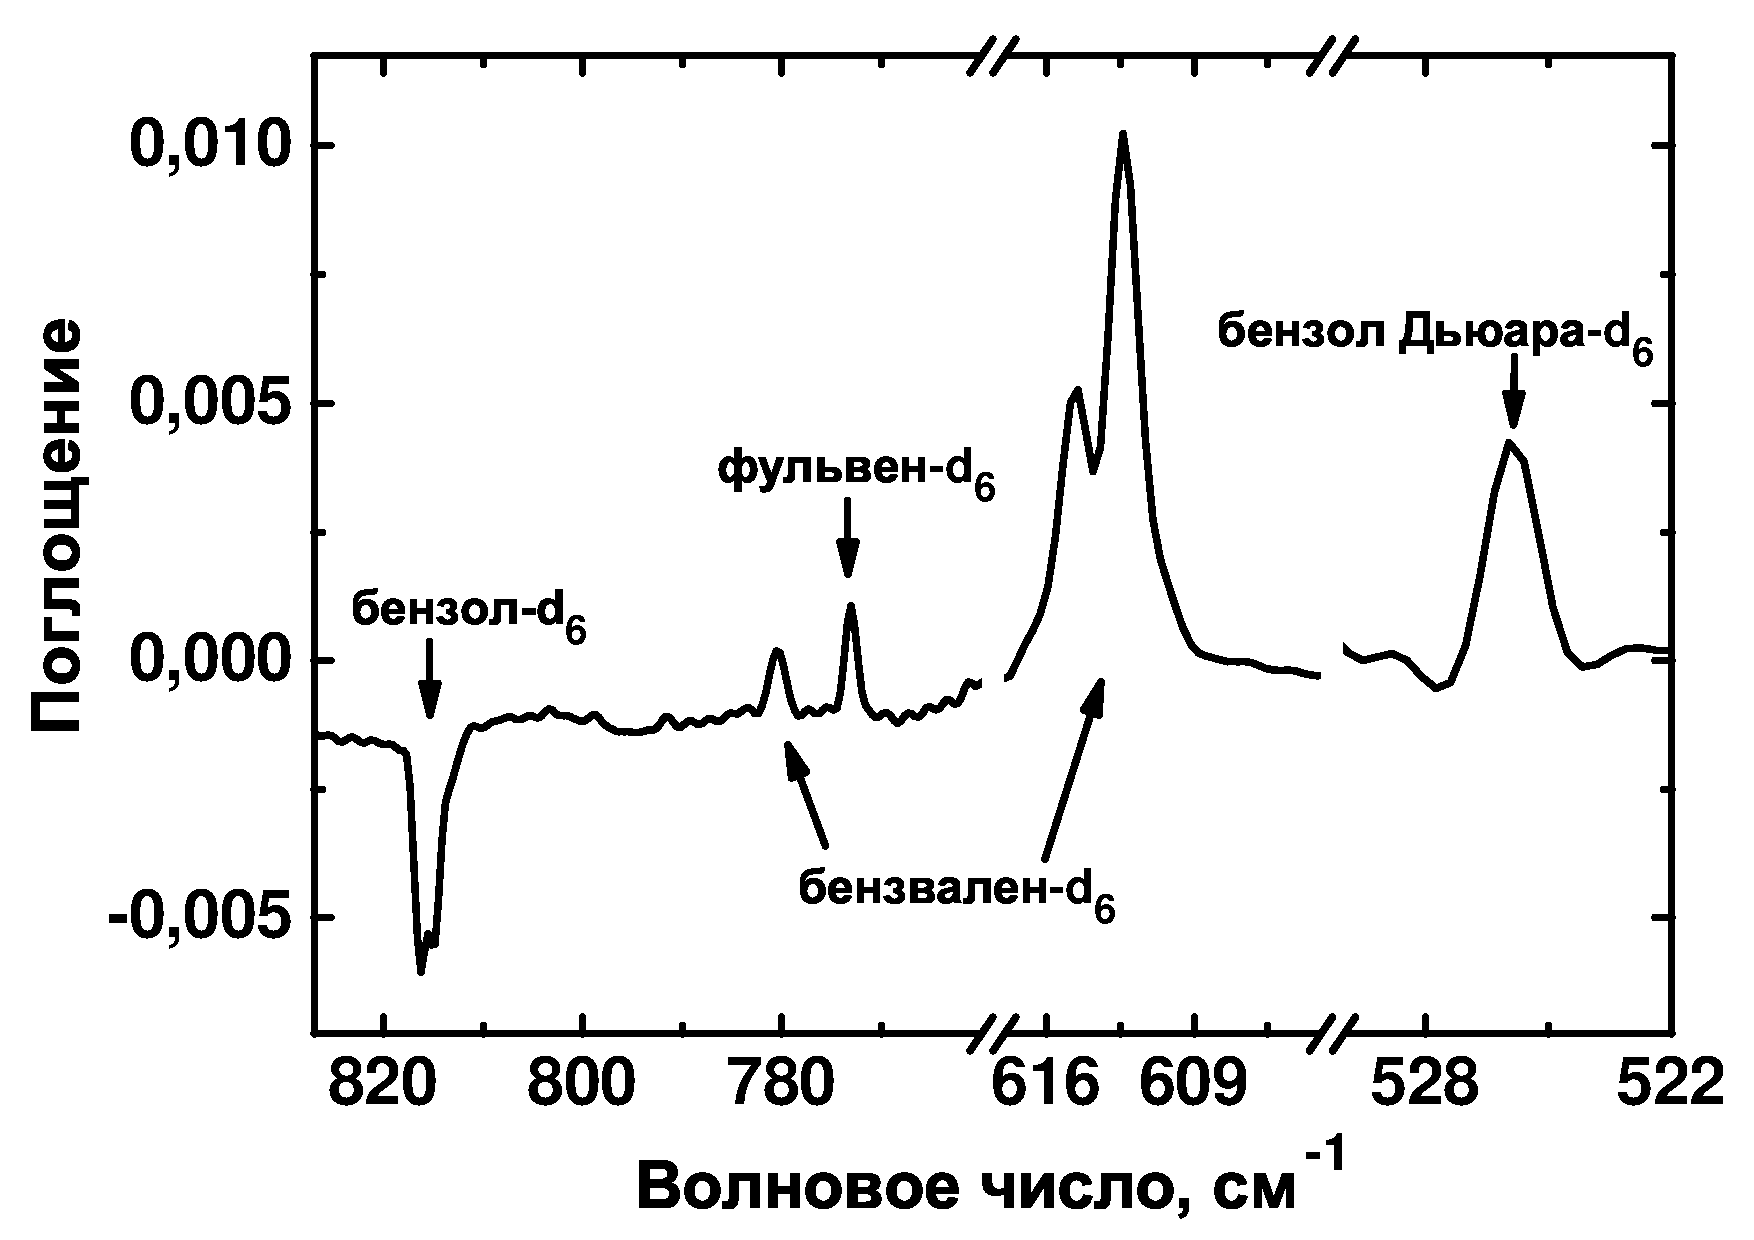
\includegraphics[width=\linewidth]{ph_sp.pdf}}
\caption{Разностный спектр фотолизованого и осаждённого образцов C$_6$D$_6$/Ar}
\label{diff}
\end{figure}

 \begin{table}[H]
\caption{Экспериментальные волновые числа (Ar) и расчётные частоты~(PBE/L2\_3) колебаний бензвалена-$d_6$~(см$^{-1}$)}
\label{benz_fr}
\begin{center}
\begin{tabular}{cc}
Ar &  Расчёт \\
\hline
612.4 & 608.5\\
614.7 & \\
640.6 & 640.7\\
642.7 & \\
780.4 & 770.5\\
\end{tabular}
\end{center}
\end{table}

 \begin{table}[H]
\caption{Экспериментальные волновые числа (Ar) и расчётные частоты~(PBE/L2\_3) колебаний бензола Дьюара-$d_6$~(см$^{-1}$)}
\label{Dewar_fr}
\begin{center}
\begin{tabular}{cc}
Ar &  Расчёт \\
\hline
519.6 & 524.4\\
525.9 & \\
631.7 & 635.3\\
654.8 & 650.2\\
657.6 & \\
733.4 & 735.3\\
\end{tabular}
\end{center}
\end{table}


Итак, проведём сравнение процессов протекающих при радиолизе и фотолизе бензола в матрицах. 
Процессы, происходящие при радиолизе бензола в матрицах можно описать следующими уравнениями:
\vspace{-2ex}
\begin{equation}\label{eq1_}
\mathrm{ 
Ng \leadsto Ng^{+\bullet}, e^-, Ng^*}
\end{equation}
\begin{equation}\label{eq2_}
\mathrm{
Ng^{+\bullet} + C_6H_6  \to (C_6H_6^{+\bullet})^* + Ng}
\end{equation}
\begin{equation}\label{eq3_}
\mathrm{
Ng^* + C_6H_6   \to C_6H_6^*  + Ng}
\end{equation}
\begin{equation}\label{eq4_}
\mathrm{
(C_6H_6^{+\bullet})^*  \to C_6H_6^{+\bullet} }
\end{equation}
\begin{equation}\label{eq6_}
\mathrm{
C_6H_6^{+\bullet}   + e^- \to C_6H_6^{**} \;(S_n, T_n)}
\end{equation}
\begin{equation}\label{eq7_}
\mathrm{
C_6H_6^*\;(C_6H_6^{**})\; (T_n)\to C_6H_5^\bullet + H^\bullet}
\end{equation}
\begin{equation}\label{eq8__}
\mathrm{
H^+ + 2Ng \to Ng_2H^+}
\end{equation}
\begin{equation}\label{eq9_}
\mathrm{
C_6H_6^*  \; (C_6H_6^{**}) \;(S_n) \to \text{фульвен}}
\end{equation}

Процессы при радиолизе C$_6$D$_6$ в матрицах аналогичны.
Необходимо подчеркнуть, что при рекомбинации КР бензола с электронами заселяются высшие синглетные и триплетные состояния (уравнение~\ref{eq6_}), при этом состояния T$_n$ являются предшественниками фенильного радикала. Другой путь его образования~--- депротонирование КР бензола~--- играет меньшую роль, так как КР~бензола не является хорошим донором протона. О потенциальной возможности протекания данного процесса говорит образование сольватированного протона (сольватированного дейтрона в случае C$_6$D$_6$) (уравнение \ref{eq8__}). Однако Ng$_2$H$^+$ и Ng$_2$D$^+$ могут возникать также при депротонировании КР продуктов радиолиза бензола.

При фотолизе излучение поглощается непосредственно молекулами бензола (уравнение~\ref{eq10_}). При этом энергии излучения (254~нм) достаточно только для возбуждения в состояние~S$_1$.

\begin{equation}\label{eq10_}
\mathrm{C_6H_6} \xrightarrow{h\nu} \mathrm{C_6H_6^* \;(S_1)} 
\end{equation}
\begin{equation}\label{eq11_}
\mathrm{
C_6H_6^* \;(S_1) \to \text{изомеры бензола}}
\end{equation}

Теоретические и экспериментальные работы по фотолизу бензола в газовой фазе предсказывают образование бензола Дьюара только из состояния S$_2$, но не из S$_1$.  Однако, ранее было показано образование бензола Дьюара из бензола при фотолизе на длине волны 254~нм в матрице аргона (см. раздел~\ref{photolysis}). Наши эксперименты указывают на то, что фотолиз дейтерированного бензола в матрице аргона протекает аналогично фотолизу недейтерированного бензола.

При радиолизе бензола в матрицах в значимых количествах стабилизируется только один из изомеров бензола (фульвен). Отсутствие бензвалена и бензола Дьюара можно объяснить тем, что эти изомеры могут образовываться в возбуждённом состоянии и не релаксировать до основного, а сразу же превращаться в бензол или фульвен (такая изомеризация известна при фотолизе, см. раздел~\ref{photolysis}). 

Таким образом, принципиально разные механизмы поглощения энергии излучения при радиолизе и фотолизе приводят к различному составу продуктов.

}





















